

% !TEX root = NotesDeCours.tex


%%%%%%%%%%%%%%%%%%%%%%%%%%%%%%%%%%%%%%%%%%%%%%%%%%%%%%%%%%%%%%%%%%%%%%%%%%%%%%%%%%%%%%%%%%


%\part{Aérodynamique à haut Reynolds}
%\setcounter{section}{7}
%\beamer@tocsectionnumber=8\relax
%\section{Aérodynamique à haut Reynolds}


%%%%%%%%%%%%%%%%%%%%%%%%%%%%%%%%%%%%%%%%%%%%%%%%%%%%%%%%%%%%%%%%%%%%%%%%%%%%%%%%%%%%%%%%%%



\begin{frame}

  \color{bleu}

  \begin{flushleft}
    
    \Large
   	\bf
    
    Mécanique des fluides 

  \end{flushleft}
  
  \ligne{3} % remplace: \noindent \thickline{0.5mm}{150}

  \begin{flushright}

    \rm

    \textrm{David} \textsc{Fabre}
    
    \vspace{3mm}
    
    IMFT / UPS
    
    Département de Mécanique
    
  %  brancher@imft.fr

  \end{flushright}

%\begin{picture}(110, 22)(-9, 5)
 \begin{center}
    \begin{picture}(100, 40)(0, -5)
    \put(0, 0){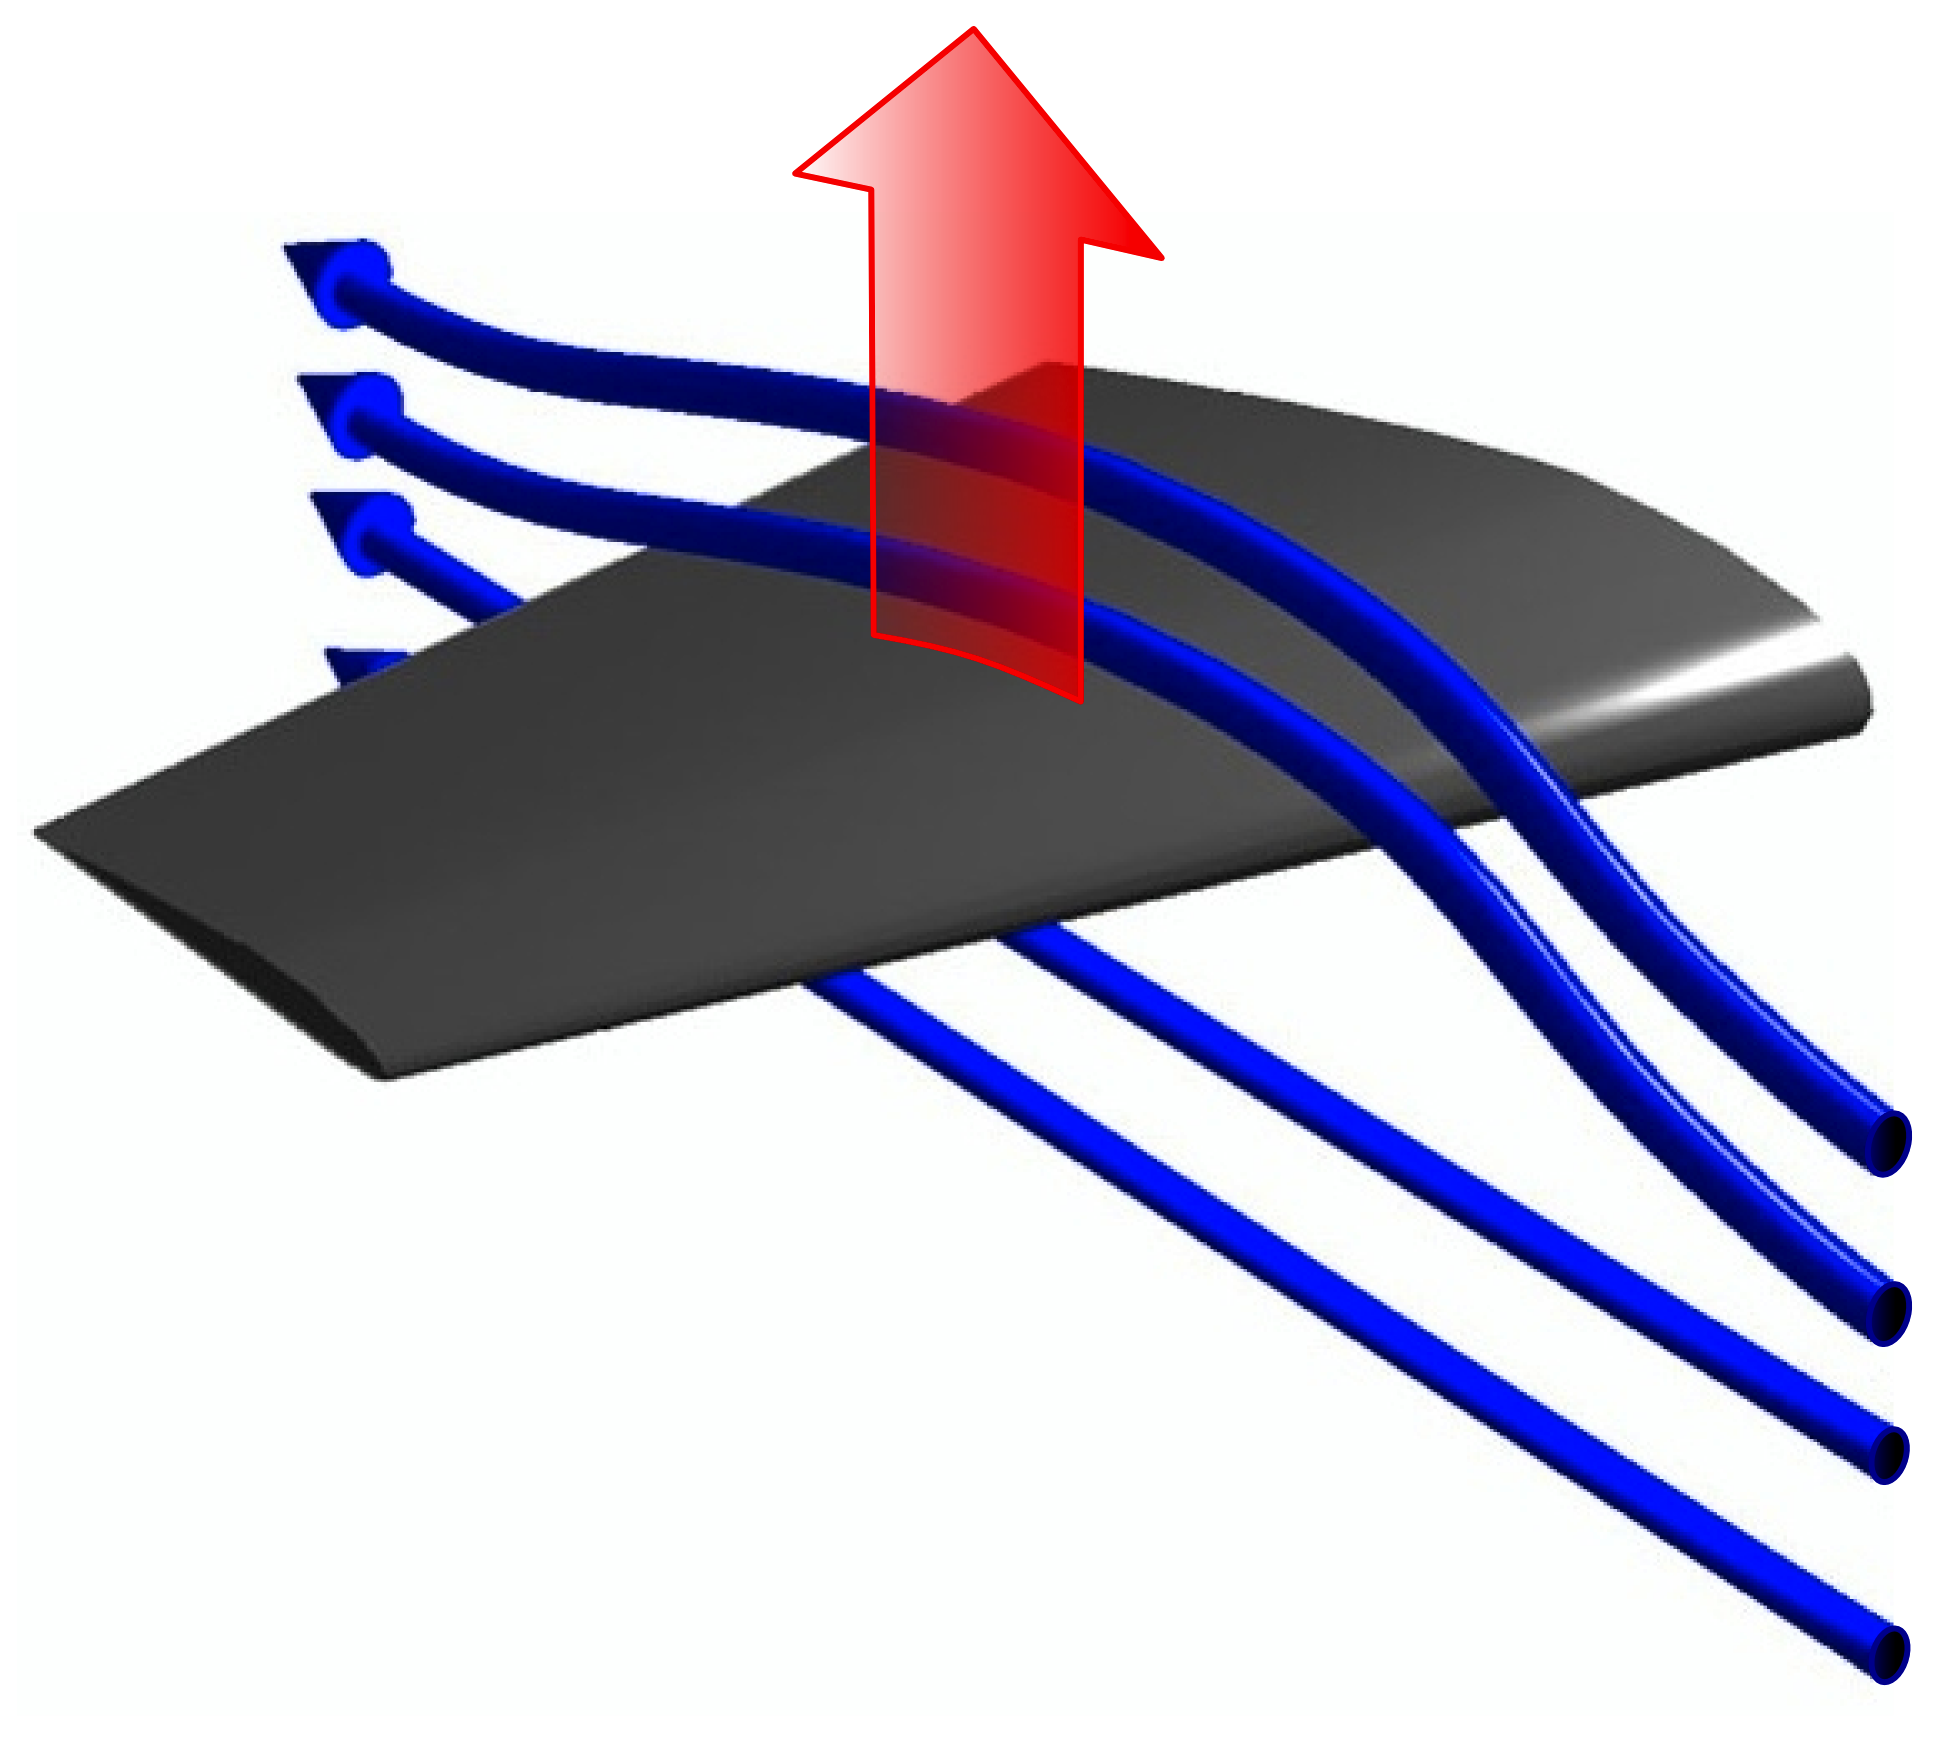
\includegraphics[width=30mm]{flow_airfoil_fliped.png}}
    \put(50, 5){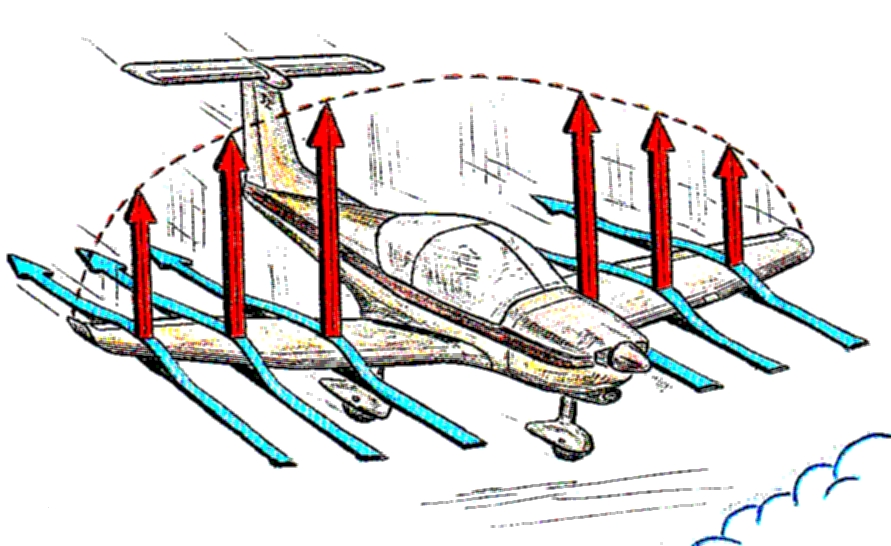
\includegraphics[width=40mm]{portance_posterized.jpg}}
   % \put(38, 28){\color{red} \bf PORTANCE}
    \end{picture}
  \end{center}


 % \put( 0, 25){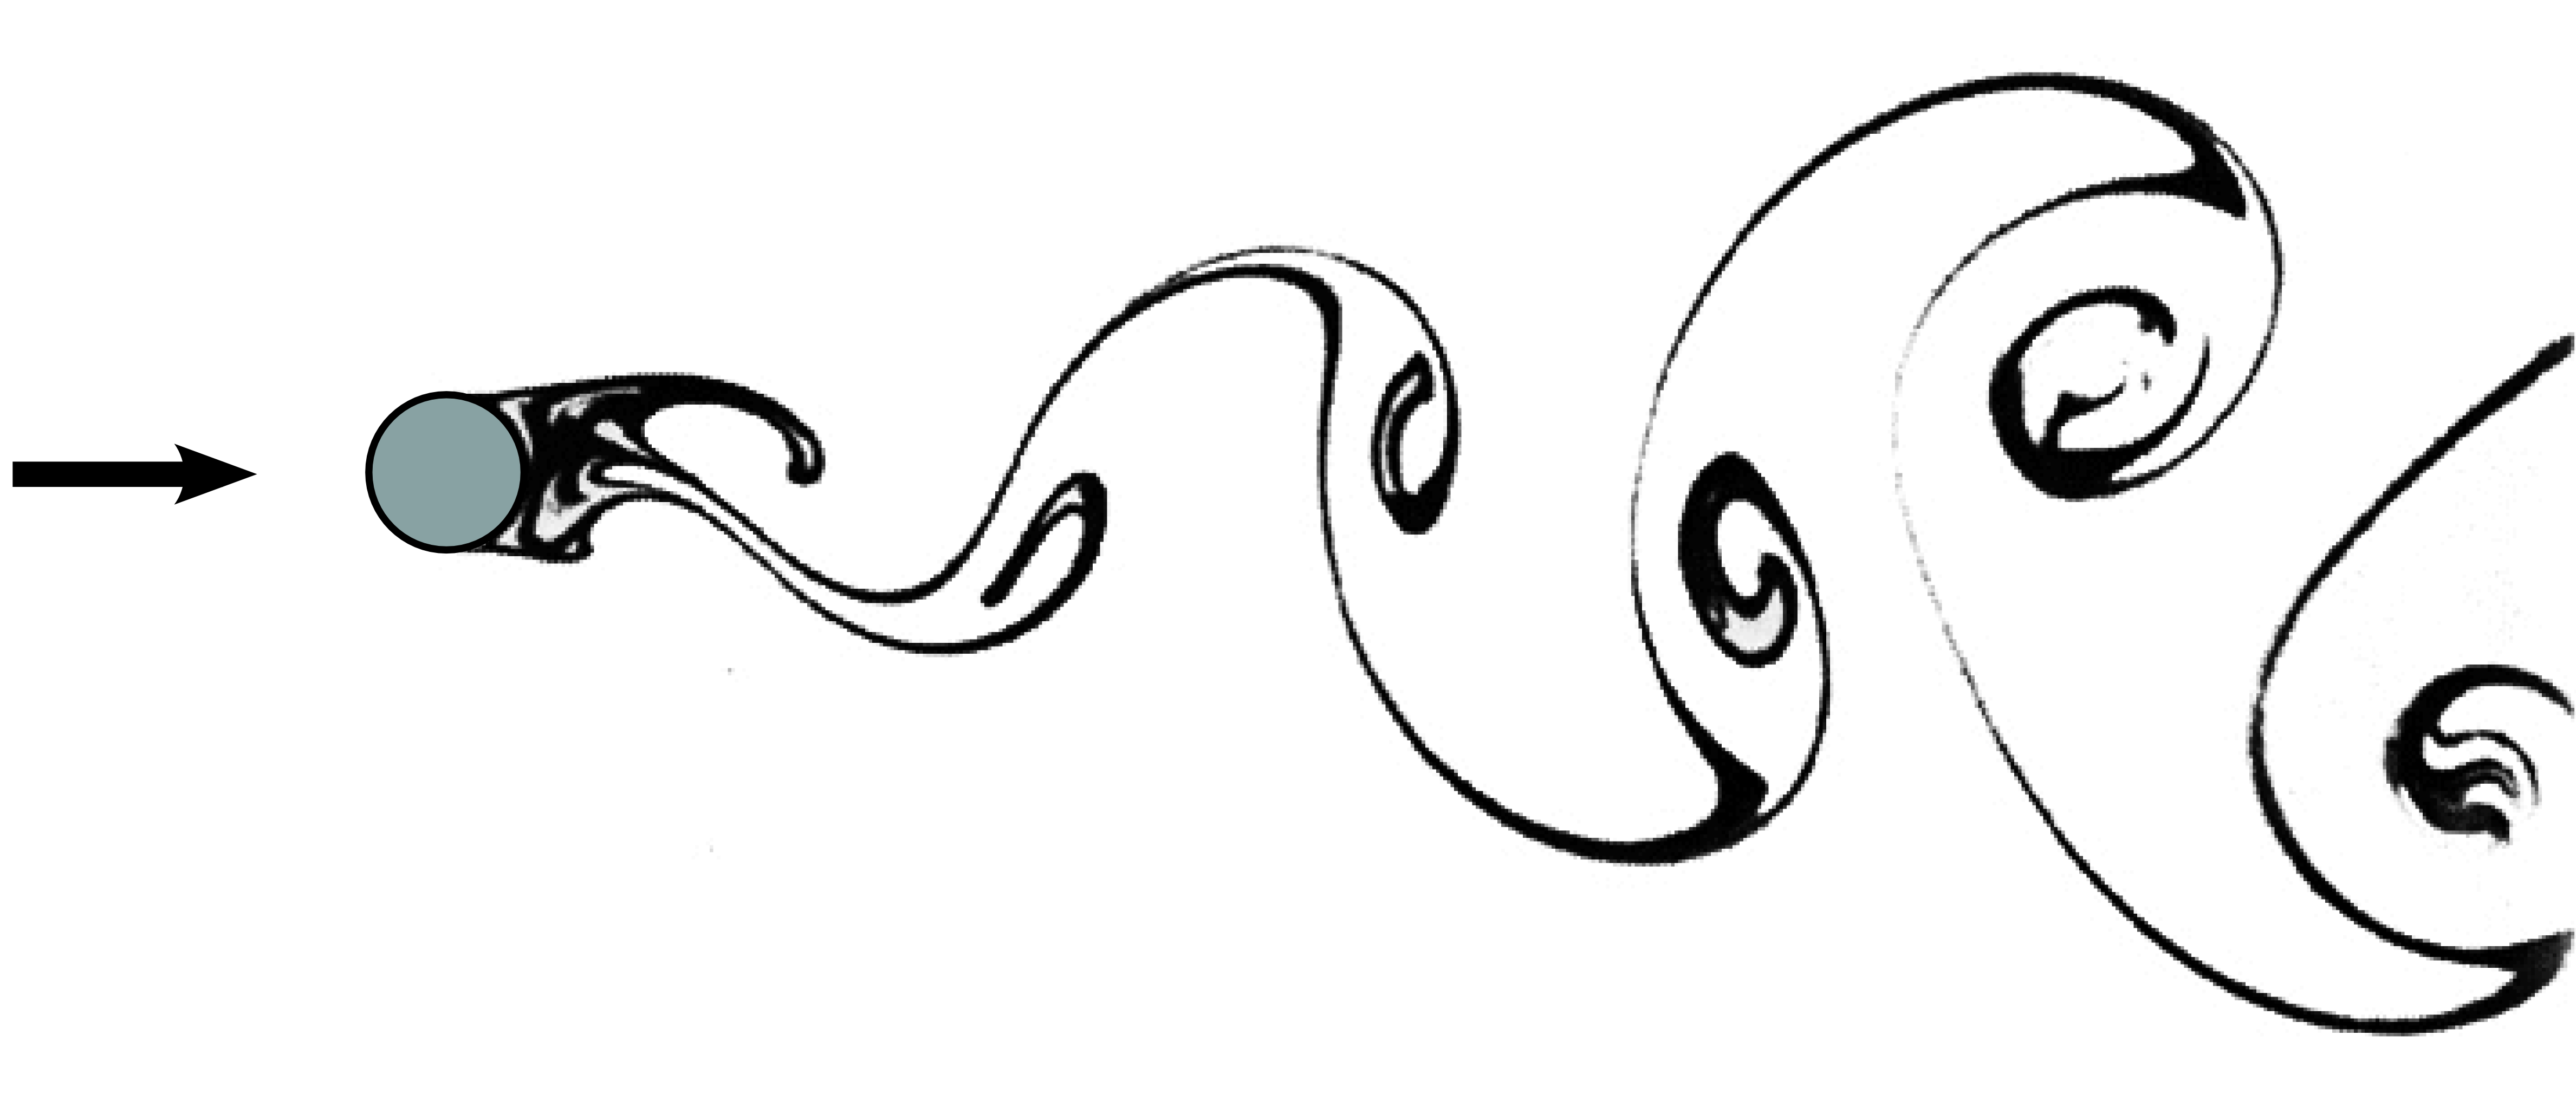
\includegraphics[width=50mm]{./Figures/Von_Karman.png}}
 % \put( 6,  0){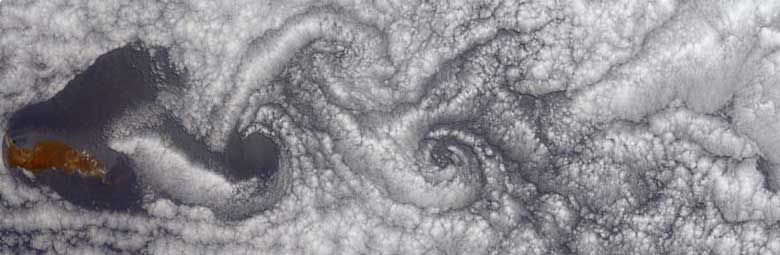
\includegraphics[width=50mm]{./Figures/VK_Guadalupe.jpg}}
 % \put( 0, 23){\color{gris} \small \rm Allée de tourbillons de Von Karman} 
  %\put( 0, 20){\color{gris} \small \rm en aval d'un cylindre à $Re=140$ (lignes d'émission).}
  %\put( 0,  -3){\color{gris} \small \rm Allée de tourbillons de Von Karman}
  %\put( 0, -6){\color{gris} \small \rm dans le sillage de l'île de Guadalupe (océan Pacifique).}
  
  
%\end{picture}

  \vspace{12mm}
  
  \begin{flushright}
    
    \Large
   	\bf
    
    8. Ecoulements potentiels et Aérodynamique à haut Reynolds

  \end{flushright}

\end{frame}

%%%%%%%%%%%%%%%%%%%%%%%%%%%%%%%%%%%%%%%%%%%%%%%%%%%%%%%%%%%%%%%%%%%%%%%%%%%%%%%%%%%%%%%%%%
% Sommaire :
%%%%%%%%%%%%%%%%%%%%%%%%%%%%%%%%%%%%%%%%%%%%%%%%%%%%%%%%%%%%%%%%%%%%%%%%%%%%%%%%%%%%%%%%%%

\part{Ecoulements Potentiels - Aérodynamique à haut Reynolds}


\section*{\bfseries 8. Ecoulements Potentiels - Aérodynamique à haut Reynolds}


%\part{Aérodynamique à haut Reynolds}
%\setcounter{section}{7}
%\beamer@tocsectionnumber=7\relax
%\section{Aérodynamique à haut Reynolds}





%%%%%%%%%%%%%%%%%%%%%%%%%%%%%%%%%%%%%%%%%%%%%%%%%%%%%%%%%%%%%%%%%%%%%%%%%%%%%%%%%%%%%%%%%%
%\section{\bfseries Aérodynamique à grand Reynolds}
%%%%%%%%%%%%%%%%%%%%%%%%%%%%%%%%%%%%%%%%%%%%%%%%%%%%%%%%%%%%%%%%%%%%%%%%%%%%%%%%%%%%%%%%%%


%\begin{frame}{Sommaire}
%
%\small
%  
%\hspace*{2mm}
%\begin{tabular}{cc}
%		%&
%  		\begin{minipage}{62mm}
%  			\tableofcontents[firstsection=-6]
%      \vspace{15mm}
%  		\end{minipage}
%  		&   
%  		\begin{minipage}{60cm}
%		  \vspace*{-5mm}  
%  			%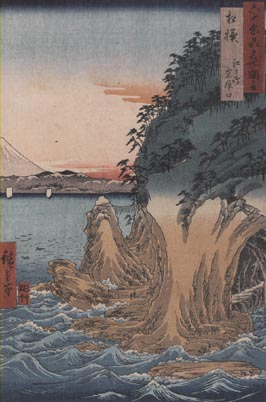
\includegraphics[width=40mm]{vagues.jpg} 
%  		\end{minipage}
%  	\end{tabular}
%
%\vspace{0mm}
%
%\end{frame}


\subsection{Ecoulements potentiels}
\subsubsection{Dynamique de la vorticité}
%------------------------------------------------------------------------------------------
\begin{frame}{Dynamique de la vorticité} \hypertarget{frame:toto}{}
%------------------------------------------------------------------------------------------

\small

\vspace{0mm}

En prenant le rotationnel de l'équation de Navier-Stokes on obtient l'équation de Helmholtz 
qui gouverne l'évolution de la vorticité $\myvec{\omega} = \myvec{rot} ( \myvec{u} ) $

\begin{equation}
	{\color{rouge}
\ddt{\myvec{\omega}} =  \dpdt{\myvec{\omega}} + \left( \mytensor{grad} \myvec{\omega} \right) \cdot  \myvec{u} 
  =  \left( \mytensor{grad} \myvec{u} \right) \cdot  \myvec{\omega} +
  \nu \Delta \myvec{\omega} \qquad }\mbox{{\color{gris}[Démonstration]}}
\end{equation}

Interprétation :  3 modes d'évolution de la vorticité

Transport, $\qquad$ Etirement , $\qquad$ Diffusion



$\longrightarrow$ La viscosité peut également être interprétée comme un phénomène de {\color{red} diffusion de la vorticité.}

Si $Re \gg 1$, la diffusion est négligeable, la vorticité est uniquement advectée et étirée.

\medskip
Conséquence {\color{red} (Théorème de Laplace)} :

Si $\myvec{\omega} = \myvec{0}$ initialement dans tout l'écoulement
et si les forces visqueuses sont négligeables, alors $\myvec{\omega}$ reste nulle.


\medskip Ce théorème justifie qu'en pratique de nombreux écoulements à grand nombre de Reynolds sont irrotationnels.



%Le terme d'étirement (présent uniquement en 3D) n'est pas un terme source mais seulement un %terme de réorientation de la vorticité. 


\end{frame}

%\end{document}


\subsubsection{Ecoulements potentiels : définition et propriétés}
%------------------------------------------------------------------------------------------
\begin{frame}{Ecoulements potentiels} \hypertarget{frame:toto}{}
%------------------------------------------------------------------------------------------

\small



\vspace{0mm}

Si $\myvec{rot}(\myvec{u}) = \myvec{0}$, alors il existe une fonction 
$\Phi$ appelée {\color{red}Potentiel des vitesses } telle que :

$$
\myvec{u} = \gradient{\Phi}
$$


\pause
Si, de plus, $div(\myvec{u}) = 0$, alors le potentiel vérifie l'équation suivante :

$$
\Delta{\Phi} = 0.
$$

Dans ce cas le calcul d'un écoulement se ramène alors à la résolution d'une équation scalaire linéaire particulièrement simple  !

\smallskip

Il existe des méthodes mathématiques puissantes pour résoudre cette équation dans un grand nombre de cas (cf. programme de Master).


\pause 
\medskip
Remarques :

\begin{itemize}
\item
 $\Phi$ est défini à une constante près, qui peut éventuellement dépendre du temps.

\pause 

\item L'hypothèse d'écoulement potentiel est une \em{hypothèse mathématique}, contrairement à l'hypothèse de régime d'écoulement inertiel qui est une hypothèse physique !
 \smallskip 
(En général les écoulements inertiels sont potentiels "loin des obstacles", mais il existe des contre-exemples !) 




\end{itemize}


\end{frame}




%------------------------------------------------------------------------------------------
\begin{frame}{Ecoulements potentiels : propriétés} \hypertarget{frame:toto}{}
%------------------------------------------------------------------------------------------

\small

Propriétés : 

\begin{itemize}
\item Les écoulements potentiels vérifient $\Delta {\myvec u} =0$ {\color{gris} [Démonstration]}. 

Ils sont donc solutions des équations d'Euler quelque soit la viscosité et donc le nombre de Reynolds !
\pause
%Rem : 
%$div(\mytensor{\tau}=\myvec{0}$, les contraintes visqueuses sont équilibrées 

 % Exemple : Ecoulement (Exercice 5.4?)
  
\smallskip
\item Réversibilité en temps  : si $\myvec{u} = \gradient (\Phi)$ est solution, alors 
$- \myvec{u} = \gradient (- \Phi)$ l'est également.
  
  \pause 
\smallskip
\item Additivité des solutions : si $\myvec{u}_1 = \gradient \Phi_1$ et $\myvec{u} _2 = \gradient \Phi_2$ 
sont deux écoulements potentiels alors 
$\myvec{u} = \gradient (\Phi_1+\Phi_2)$ l'est également.

\pause
\medskip 
Remarque importante : non-additivité des pressions !

($p \ne p_1 + p_2$)



\end{itemize}

\pause

\bigskip



\medskip

Limitation : On montre qu'un écoulement potentiel stationnaire autour d'un obstacle génère une force
de traînée nulle sur celui-ci ! (Paradoxe de d'Alembert).

\smallskip

En revanche l'écoulement potentiel autour d'un objet bidimensionnel (par exemple un profil d'aile) peut conduire à une force de portance non nulle.

\smallskip

%$\rightarrow$ La théorie des profils portants s'appuie sur le modèle potentiel (programme de M1).

\vspace{0mm}
\end{frame}



\begin{frame}{Potentiels des vitesses et fonction de courant}

Pour les écoulements bidimensionnels, le \textcolor{red}{potentiel des vitesses} $\Phi$ et la 
 \textcolor{red}{fonction de courant} $\Psi$ jouent des rôles voisins.

 \vspace{.5cm} 
 $$
 \rot \vec{u}  =  \vec{0} \qquad \longrightarrow \quad \exists   \Phi \mbox{ t.q. } \vec u = \gradient \Phi
 $$
 Si de plus $\divergence (\vec{u}) = 0$, $\qquad  \longrightarrow \quad$ $\Delta \Phi = 0$.


 $$
 \divergence ( \vec{u})  =  0 \qquad  \longrightarrow \quad \exists   \Psi \mbox{ t.q. } \vec u = \rot (\Psi \vec{e_z} )
 $$
 Si de plus $\rot \vec{u} = \vec{0} $, $\qquad  \longrightarrow \quad$ $\Delta \Psi = 0$.
 
 \vspace{.5cm}
 
 Pour les écoulements irotationnels et incompressibles, on peut utiliser les 2. Dans ce cas le lignes iso-potentielles $(\Phi = Cte)$  et les lignes de courant   $(\Psi = Cte)$ forment 
 deux réseaux de courbes orthogonales.
 
 
 \vspace{.3cm}

 
 On peut de plus combiner ces deux outils en un unique potentiel complexe défini par $f(x,y) = \Psi(x,y) + i \psi(x,y)$, qui a des propriétés mathématiques très utiles (cf. programme de M1).
 
\end{frame}
 


\subsubsection{Second théorème de Bernoulli}
%------------------------------------------------------------------------------------------
\begin{frame}{Second théorème de Bernouilli pour les écoulements potentiels} \hypertarget{frame:toto}{}
%------------------------------------------------------------------------------------------

\small

Sous les hypothèses suivantes :
\medskip

$(a)$ Ecoulement incompressible,
 

$(b)$ Champ de gravité uniforme,

%Forces volumiques conservatives % $\myvec{g} = -\gradient ( {\mathcal U})$ (en général 
%${\mathcal U} = g z$).

$(e)$ Ecoulement potentiel (c.a.d. irrotationnel),

\medskip

La quantité 
$
p+\rho g z + \rho |\myvec{u}|^2/2 +\rho \frac{\partial \Phi}{\partial t}
$
est {\em uniforme} dans tout l'écoulement. {\color{gris}[Démonstration]}

\pause
\medskip

On note aussi (formellement) : 
$$
\frac{p}{\rho} + g z + |\myvec{u}|^2/2 + \frac{\partial \Phi}{\partial t} = C^{te}(t)
$$

\bigskip

Cette version du théorème permet de calculer très facilement la pression 
(et donc les forces exercées sur un obstacle) dans un écoulement potentiel, si l'on connait la valeur de la pression en {\bf un} point du domaine (choisi par exemple "loin des obstacles" ou "sur une surface libre").

\pause
\medskip

Remarques : 
\begin{itemize}
\item Si l'écoulement est stationnaire, alors la  $C^{te}$ est habituellement déterminée en fonction des conditions à l'infini.

\item Dans le cas instationnaire, la $C^{te}(t)$ peut être choisie arbitrairement à zéro
(le potentiel est lui aussi défini à une $C^{te}(t)$ près).


\end{itemize}


\vspace{0mm}
\end{frame}


\subsubsection{Ecoulements potentiels : exemples}


%\begin{frame}{Ecoulement autour d'un cylindre : généralités}
%\small

%\end{frame}


%------------------------------------------------------------------------------------------
\begin{frame}{Exemple 1 : cylindre} \hypertarget{frame:toto}{}
%------------------------------------------------------------------------------------------

\small


Exemple important : { \bf Ecoulement potentiel autour d'un cylindre}.

{\color{vert}( Exercice 8.0, a traiter en exercice préparatoire)} 

\medskip

Considérons l'écoulement stationnaire, bidimensionnel autour d'un cylindre de rayon $a$
dans un fluide de masse volumique $\rho$ (on néglige la gravité, ou on travaille avec la pression motrice).
\medskip

Deux solutions élémentaires :

\begin{itemize}
\item Solution symétrique $\Phi_s = x \left( 1 + \frac{a^2}{x^2+y^2} \right)  
\equiv \left(r + \frac{a^2}{r} \right) \cos \theta$  

\item Solution antisymétrique $\Phi_a = arctan( y/x) \equiv \theta$ 

\end{itemize}
%\medskip

\pause

\begin{itemize}

\item La superposition des deux, c.a.d. $\Phi = U \Phi_s + \frac{\Gamma}{2 \pi} \Phi_a$, est également solution.

\end{itemize}

\medskip

%$\Phi = U \Phi_s + \Gamma \Phi_a$ est également solution.

%{\color{vert}Exercice 8.0 (a traiter en exercice préparatoire) :} 

Montrer que la force exercée sur le cylindre par cet écoulement (par unité de longueur dans la direction transverse) est dans la direction $y$ et a pour intensité 

$${\color{orange} F_y =    - \quad \rho \Gamma U }$$ 


\medskip

{\color{vert}Démonstrations :}

$(i)$ Calcul direct : par calcul de la pression $p(r,\theta)$ puis intégration sur la surface.

$(ii)$ Calcul indirect : par bilan de quantité de mouvement sur un volume de contrôle judicieusement choisi. 

\pause
\smallskip Remarque : ce résultat est généralisable quelque soit la forme de l'obstacle !

\textcolor{orange}{Théorème de Kutta-Joukowski}



\vspace{0mm}
\end{frame}

%
%%------------------------------------------------------------------------------------------
%\begin{frame}{Ecoulements potentiels : exemples} \hypertarget{frame:toto}{}
%%------------------------------------------------------------------------------------------
%
%\small
%Exemple 1 (classique et très important) :
%
%\medskip
%Ecoulement stationnaire, bidimensionnel autour d'un cylindre de rayon $a$.
%
%\medskip
%
%Deux solutions élémentaires :
%
%\begin{itemize}
%\item Solution symétrique $\Phi_s = x \left( 1 + \frac{a^2}{x^2+y^2} \right)  
%\equiv \left(r + \frac{a^2}{r} \right) \cos \theta$  
%
%\item Solution antisymétrique $\Phi_a = arctan( y/x) \equiv \theta$ 
%
%\end{itemize}
%\medskip
%
%\pause
%
%\begin{itemize}
%
%\item La superposition des deux, c.a.d. $\Phi = U \Phi_s + \frac{\Gamma}{2 \pi} \Phi_a$, est également solution.
%
%\end{itemize}
%
%\medskip
%
%%$\Phi = U \Phi_s + \Gamma \Phi_a$ est également solution.
%
%{\color{vert}Exercice :} Montrer que la force exercée sur le cylindre par cet écoulement (par unité de longueur dans la direction transverse) est dans la direction $y$ et a pour intensité 
%
%$$F_y \quad = \quad {\color{blue} \pi \rho g a^2} \quad  {\color{red} - \quad \rho \Gamma U }$$ 
%
%\medskip
%
%Les deux termes correspondent à la {\color{blue} poussée d'Archimède} et la {\color{red} portance aérodynamique}.
%
%
%
%\vspace{0mm}
%\end{frame}
%

%-----------------------------------------------------------------------------------------
\begin{frame}{Exemple 2 }
%-----------------------------------------------------------------------------------------
Exemple 2  :

\medskip

Oscillations dans un tube en U de longueur $L$ et section $S$.


\bigskip


http://ressources.unisciel.fr/mecaflux/co/Chap5\_Exo2.html


\bigskip

{\color{vert}{Exercice : }}

Montrez que si les oscillations sont de faible amplitudes, la période d'oscillation est
$T = 2\pi \sqrt{\frac{L}{2g}}$


\vspace{0mm}



\end{frame}

  

%\end{document}
%
%
%%\subsection{Rappels}
%\begin{frame}{Rappels : Vorticité} 
%\small
%
%Définition : $\myvec{\omega}  = \rot ( \myvec{u})$ est appelé le {\em vecteur vorticité}.
%
%\smallskip
%\pause
%
%En  2D :
% $\myvec{\omega} = \omega_z \myvec{e}_z, \quad  \omega_z = \left( \ddp{v}{x}-\ddp{u}{y} \right)$
%
%\smallskip
%\pause
%
%Interprétation : $\myvec{\omega}/2$ (parfois appelé "vecteur tourbillon") est le taux de rotation "intrinsèque" des particules fluides (cf. chapitre cinématique).
%
%\smallskip
%\pause
%
%Propriété importante : sur une paroi plane (ou faiblement courbée) 
% $\myvec{\omega}$ est directement relié à la contrainte visqueuse :
% 
% $$
% \tau_{xy} = 2 \mu D_{xy} = - \mu \omega_z
% $$
% 
%
%\end{frame}
%
%\begin{frame}{Rappels : Dynamique de la vorticité} 
%\small
%
%
%En prenant le rotationnel de l'équation de Navier-Stokes on obtient l'équation de Helmholtz 
%qui gouverne l'évolution de la vorticité $\myvec{\omega} = \myvec{rot} ( \myvec{u} ) $
%
%\begin{equation}
%	{\color{rouge}
%  \dpdt{\myvec{\omega}} + \left ( \myvec{u} \cdot \gradient{} \right ) \myvec{\omega}
%  =  \mytensor{grad} \myvec{u} \cdot  \myvec{\omega} +
%  \nu \Delta \myvec{\omega} \qquad }\mbox{{\color{gris}[Démonstration]}}
%\end{equation}
%
%Interprétation :  3 modes d'évolution de la vorticité
%
%Transport, $\qquad$ Etirement , $\qquad$ Diffusion
%
%\medskip
%
%$\longrightarrow$ La viscosité peut également être interprétée comme un phénomène de {\color{red} diffusion de la vorticité.}
%
%Si $Re \gg 1$, la diffusion est négligeable, la vorticité est uniquement advectée et étirée.
%
%\medskip
%Conséquence {\color{red} (Théorème de Laplace)} :
%
%Si $\myvec{\omega} = \myvec{0}$ initialement dans tout l'écoulement
%et si les forces visqueuses sont négligeables, alors $\myvec{\omega}$ reste nulle.
%
%
%\medskip Ce théorème justifie qu'en pratique de nombreux écoulements à grand nombre de Reynolds sont irrotationnels.
%
%
%
%\end{frame}
%
%\begin{frame}{Rappels : Ecoulements potentiels} 
%\small
%
%\small
%
%
%\vspace{0mm}
%
%
%
%Si $\myvec{rot}(\myvec{u}) = \myvec{0}$, alors il existe une fonction 
%$\Phi$ appelée {\color{red}Potentiel des vitesses } telle que :
%
%$$
%\myvec{u} = \gradient{\Phi}
%$$
%
%
%
%
%\pause
%Si, de plus, $div(\myvec{u}) = 0$, alors le potentiel vérifie l'équation suivante :
%
%$$
%\Delta{\Phi} = 0.
%$$
%
%Dans ce cas le calcul d'un écoulement se ramène alors à la résolution d'une équation scalaire linéaire particulièrement simple  !
%
%\smallskip
%
%Il existe des méthodes mathématiques puissantes pour résoudre cette équation dans un grand nombre de cas (cf. programme de Master).
%
%
%\pause 
%\medskip
%Quelques propriétés :
%
%
%\begin{itemize}
%\pause 
%
%\item
%Pour l'écoulement autour d'un objet 3D "sans trou" la solution est unique.
%
%\item 
%Pour l'écoulement autour d'un profil 2D, la solution est définie à une constante près (circulation $\Gamma$).
%
%%\smallskip
%%Pour les écoulements bidimensionnels, la fonction potentiel $\Phi$ et la fonction de courant 
%%$\psi$ introduite dans le chapitre cinématique jouent un rôle voisin.
%%\smallskip
%
%%On montre que les courbes isopotentielles ($\Phi = C^{te}$) et les lignes de courant 
%%$(\psi = C^{te})$ forment des reseaux de courbes orthogonales.
%
%\item 
%On peut déduire directement la pression de $\Phi$ par le second théorème de Bernouilli 
%
%
%
%\item Paradoxe de d'Alembert : la force de traînée exercée par l'écoulement potentiel stationnaire 
%sur un objet de forme quelconque est nulle !
%
%
%\end{itemize}
%
%
%\end{frame}


\subsection{Aérodynamique à haut Reynolds}

\subsubsection{Modélisation générale}

\begin{frame}{Ecoulement autour d'un obstacle à haut Re : modélisation} 
\small

$$
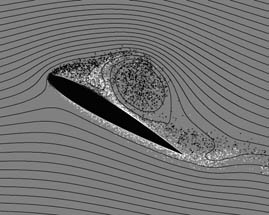
\includegraphics[width=35mm]{airfoil3.jpg}
$$

A grand Reynolds ($Re \gtrsim 10^3$), 
l'écoulement autour d'un obstacle se décompose en général en plusieurs domaines :

\begin{itemize}

\item Loin de l'obstacle : écoulement inertiel et irrotationnel (Potentiel).

La pression peut être déterminée à l'aide de Bernouilli.
%\smallskip
\pause 

\item zones décollées : écoulement inertiel mais rotationnel.

(Bernoulli inutilisable; en général la pression est quasi-uniforme dans ces zones). 

%\smallskip
\pause 
\item En proche paroi : Couches limites d'épaisseur $\delta \ll L$ à l'intérieur desquelles l'effet de la viscosité est dominant.
%\smallskip
\pause 

\item Sillage : viscosité dominante.

\end{itemize}

Remarques : 

Pour $Re \gtrsim 10^4 $ le sillage et les les zones de recirculation deviennent en général turbulentes.

Pour $Re \gtrsim 10^6 $ les couches limites deviennent également turbulentes.

\end{frame}


\begin{frame}{Ecoulement autour d'un obstacle à haut Re : Calcul des forces} 
\small

$$
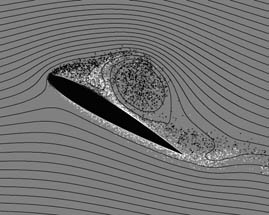
\includegraphics[width=35mm]{airfoil3.jpg}
$$

$$
\myvec{F} = \int_S (-p \myvec{n} + \mytensor{\tau}\cdot \myvec{n} ) dS
$$

On montre que (dans un fluide non pesant) la force exercée par le fluide sur l'objet peut être décomposée en 2 termes :
$$
\myvec{F} = \myvec{F}_{\hat{p}} + \myvec{F}_{v}
$$


\begin{itemize}
\item $\myvec{F}_{\hat{p}} = - \int_S \hat{p} \myvec{n} dS $ est la force due à la pression 
"motrice" et peut être calculée a partir de la solution "extérieure" inertielle,
 
%\item $ \myvec{F}_{\cal A}$ est la poussée d'Archimède qui contient l'effet de la gravité.

\item $ \myvec{F}_{v} = \int_S \mytensor{\tau}\cdot \myvec{n}  dS$ peut être calculée a partir de la solution "intérieure" dans la couche limite.

\end{itemize}

\underline{Remarque :} 

Dans un fluide pesant, il convient d'ajouter un troisième terme 
 est la poussée d'Archimède $ \myvec{F}_{\cal A}$.  qui contient l'effet de la gravité
(démo : en introduisant la pression motrice $\hat p$ ; cf. chapitre 5).



\end{frame}






\subsubsection{Exemple 1 : le cylindre}

\begin{frame}{Ecoulement autour d'un cylindre : résultats théoriques}
%\small
%\begin{picture}(25, 30)(10, -5)
%\put(30, 0){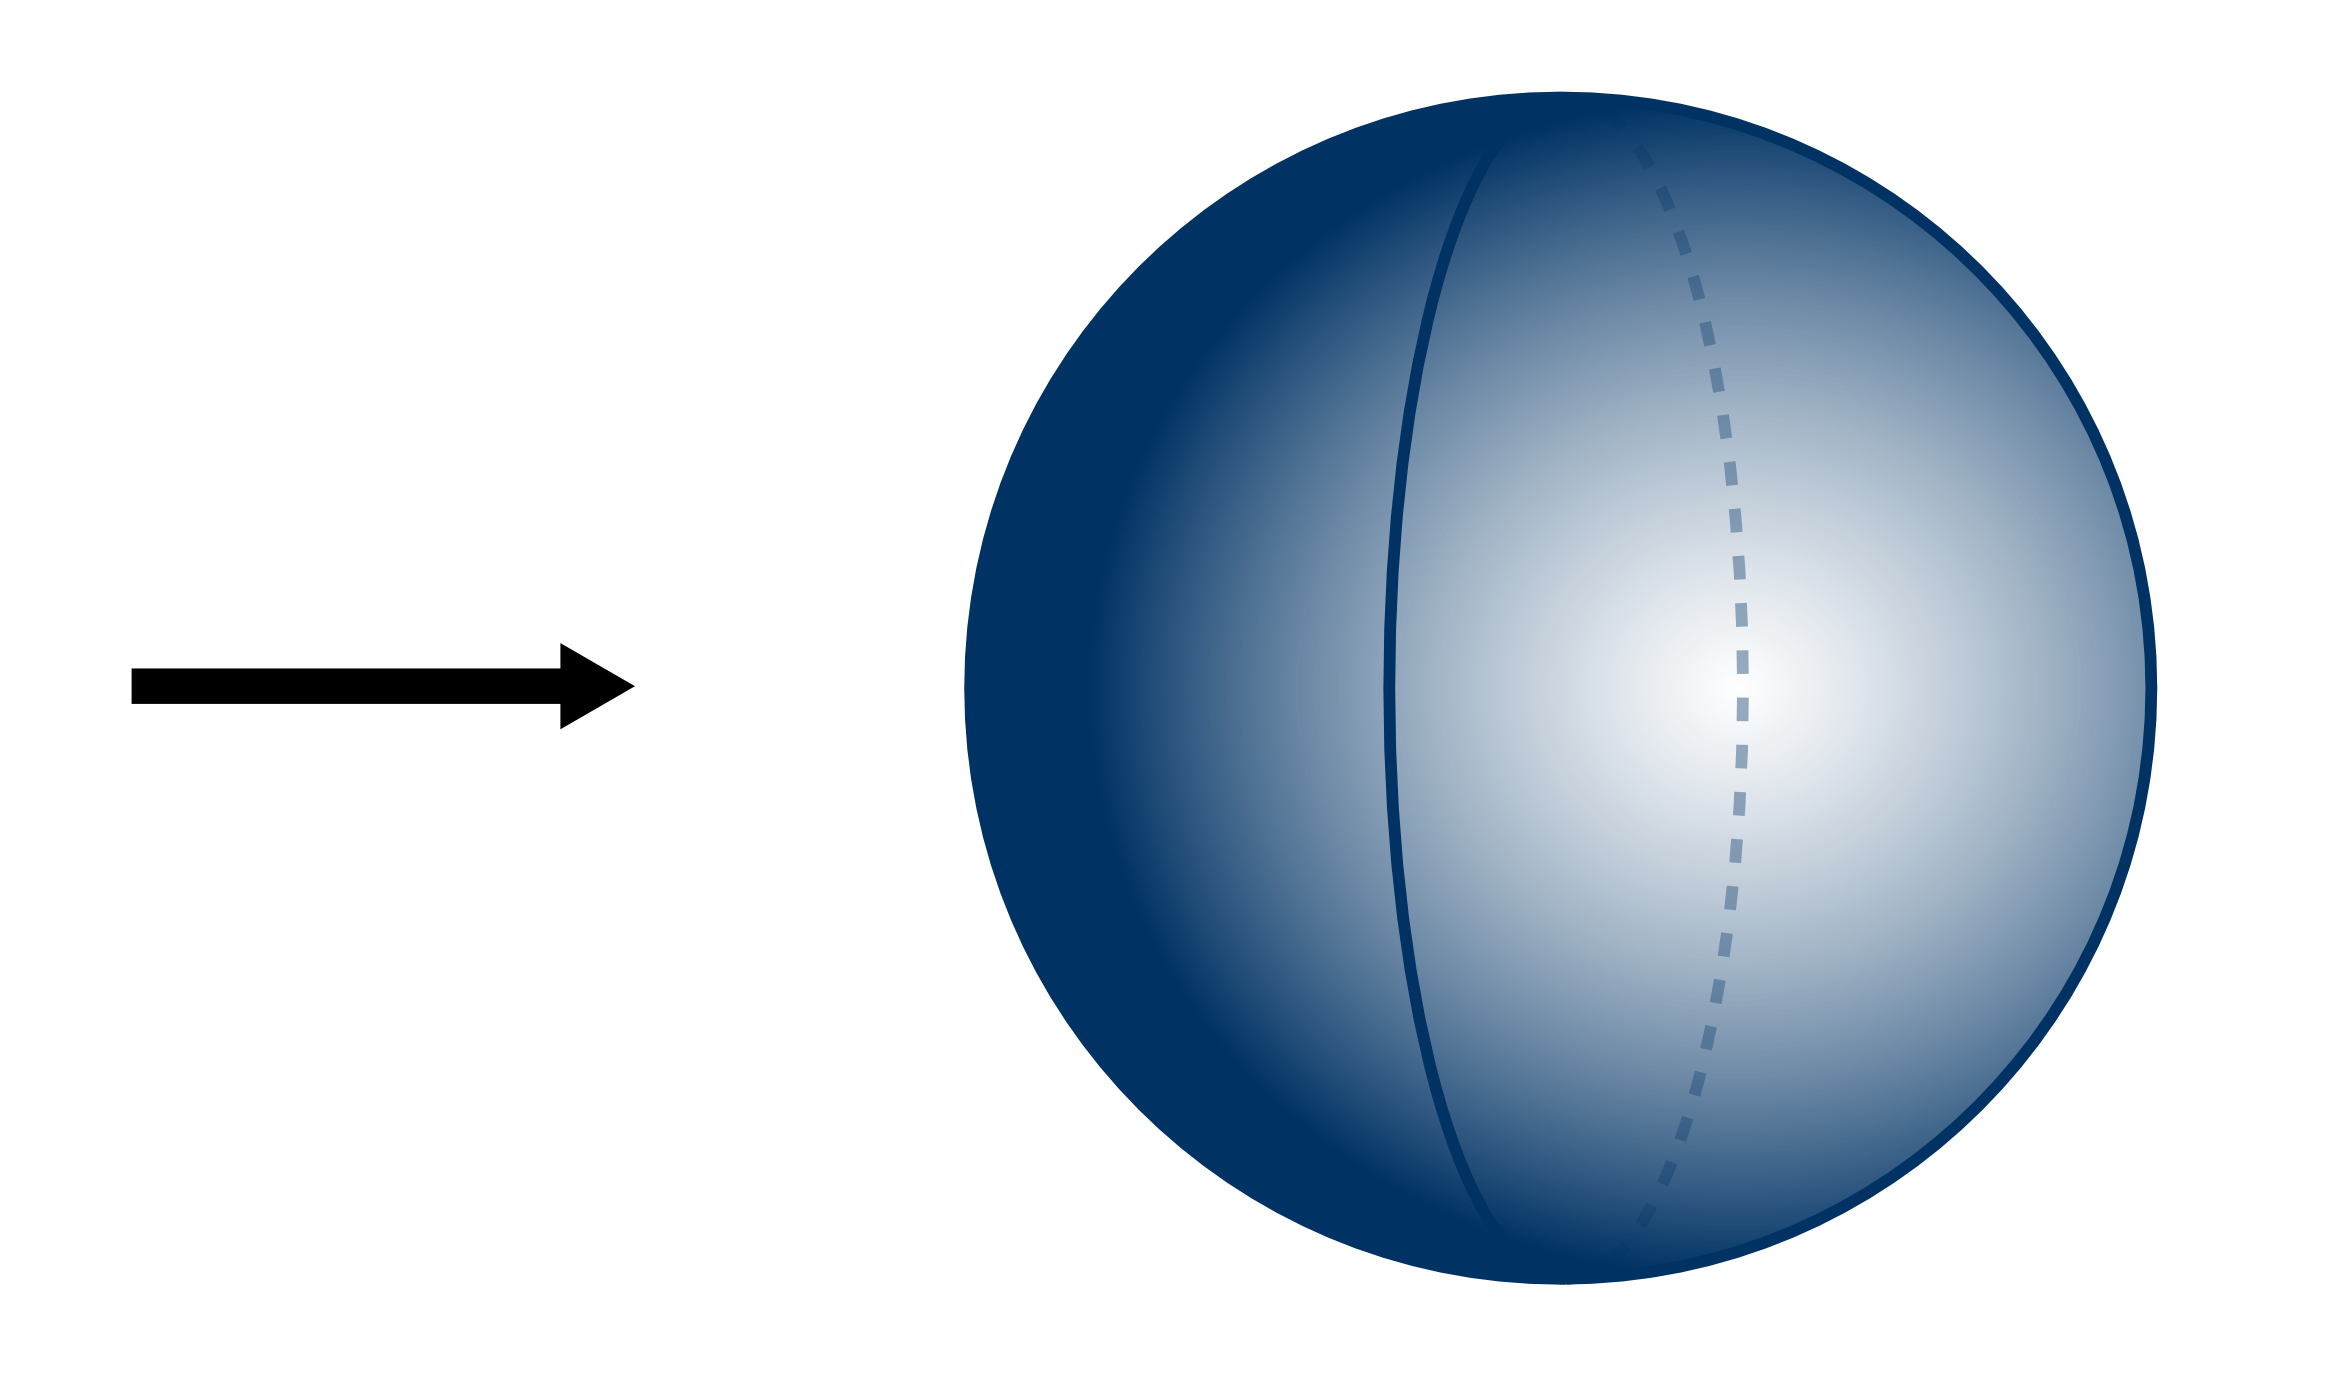
\includegraphics[width=25mm]{sphere.png}}
%		\put(47, 8){\color{red} \vector(1, 0){10}}
%		\put(60, 8){\color{red} $F_x$}
%\end{picture}


\begin{itemize}
\item Régime de Stokes ($Re = 0$) :
Il n'existe pas de solution des équations de Stokes bidimensionnelles autour d'un cylindre !
(Paradoxe de Stokes)

\item Cas des faibles nombres Reynolds :
$F_x = \frac{1}{2} \rho S C_x U^2 $
%\smallskip
%Force associée : $F_x = $
%\smallskip
avec :
$ 
C_x = \mathcal{O} \left(Re^{-1} \log Re \right)
$

\medskip 
\pause 
\item Cas potentiel  (cf. TD exercice préparatoire ) 

Il existe une solution potentielle NON UNIQUE.

 $F_x = 0$ (paradoxe de d'Alembert).

 
\end{itemize}


\end{frame}



%\end{document}
%\begin{frame}{Ecoulement autour d'un cylindre : généralités}
%\small

%\end{frame}


%------------------------------------------------------------------------------------------
\begin{frame}{Ecoulement "réel" autour d'un cylindre : cas non tournant}  \hypertarget{frame:toto}{}
%------------------------------------------------------------------------------------------

\small

Exemple pour Re = 200 :
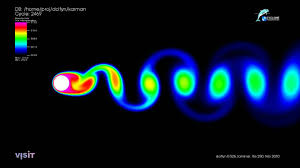
\includegraphics[width=80mm]{VonKarman_Cylindre.jpg}


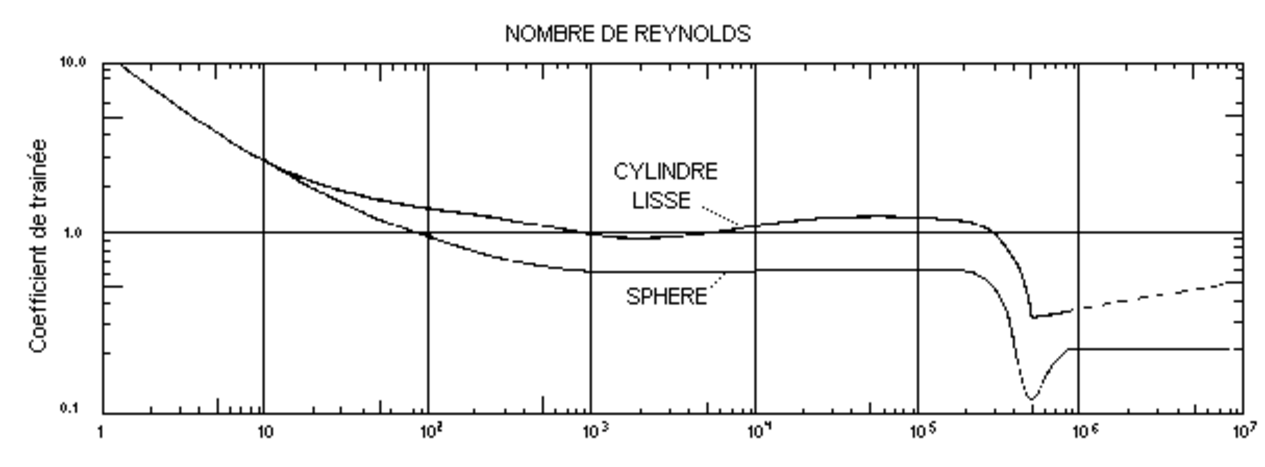
\includegraphics[width=60mm]{Cx_Cylindre_Sphere.pdf}


\end{frame}






%------------------------------------------------------------------------------------------
\begin{frame}{Ecoulement "réel" autour d'un cylindre : cas tournant}  \hypertarget{frame:toto}{}
%------------------------------------------------------------------------------------------

\small


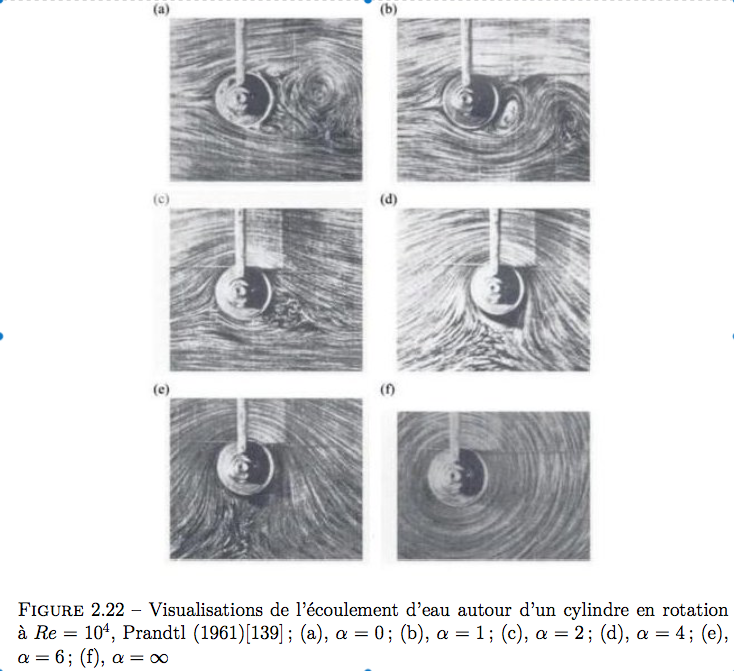
\includegraphics[width=80mm]{Cylindre_Tournant_Prandtl.png}


\end{frame}






%------------------------------------------------------------------------------------------
\begin{frame}{Application : turbovoile ou rotor "Fletner"} \hypertarget{frame:toto}{}
%------------------------------------------------------------------------------------------

\small

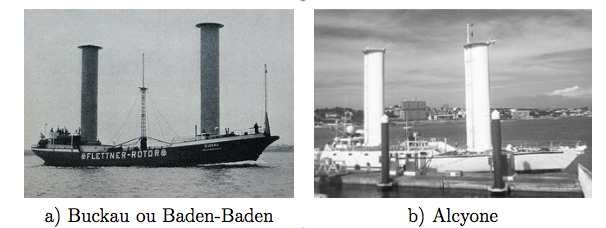
\includegraphics[width=80mm]{Alcyone.png}


\end{frame}



\subsubsection{Exemple 2 : la sphère}


%-----------------------------------------------------------------------------------------



\begin{frame}{Ecoulement autour d'une sphère : résultats théoriques}
\small
\begin{picture}(25, 30)(10, -5)
\put(30, 0){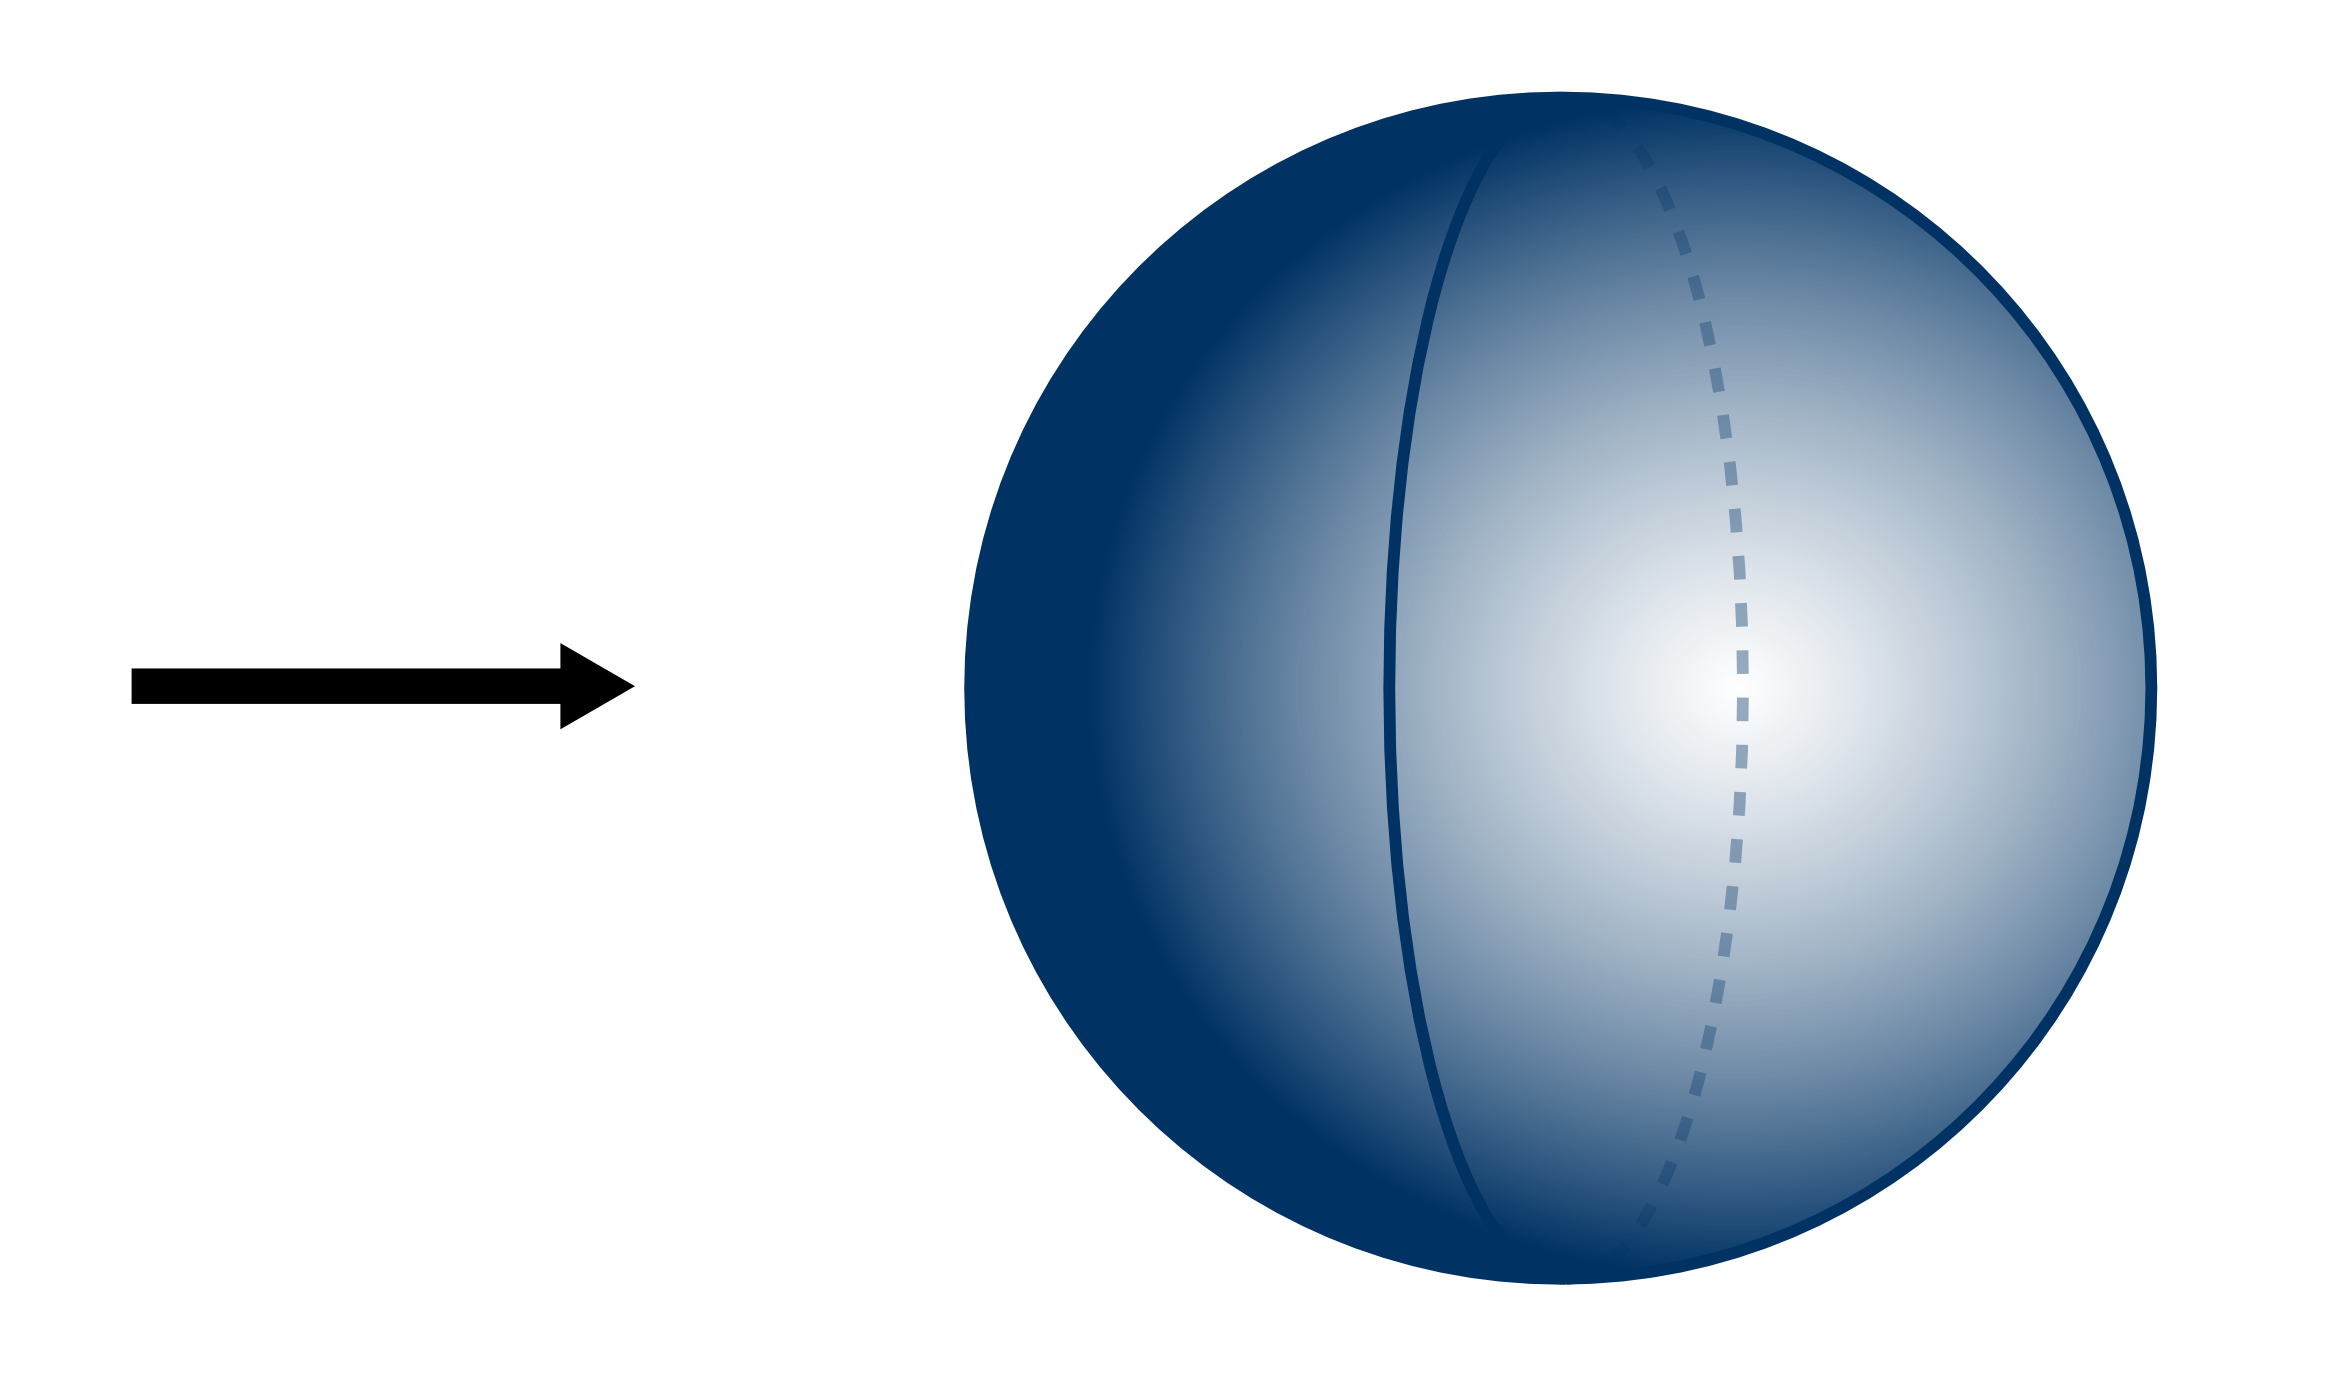
\includegraphics[width=25mm]{sphere.png}}
		\put(47, 8){\color{red} \vector(1, 0){10}}
		\put(60, 8){\color{red} $F_x$}
\end{picture}

Il existe une solution exacte dans deux cas :

\begin{itemize}
\item Régime de Stokes ($Re\ll 1$) : (cf. Chap. 6).

\smallskip
Force associée : $F_x = 6 \pi \mu a U$

\smallskip
c'est à dire :
$ 
C_x = \frac{24}{Re}
$

\medskip 
\pause
\item Solution potentielle  (cf. TD).

\smallskip
$\Phi(r,\theta) = U \left( r + \frac{a^3}{2 r^2} \right) \cos \theta$

\smallskip
Force correspondante : $\myvec{F} = \myvec{0}$ (Paradoxe de d'Alembert).

\end{itemize}


\end{frame}

%-----------------------------------------------------------------------------------------
\begin{frame}{Obstacle non profilé : la sphère}
%-----------------------------------------------------------------------------------------

\small

\begin{center}
	\begin{picture}(95, 60)(10, -5)
		\put(20, 0){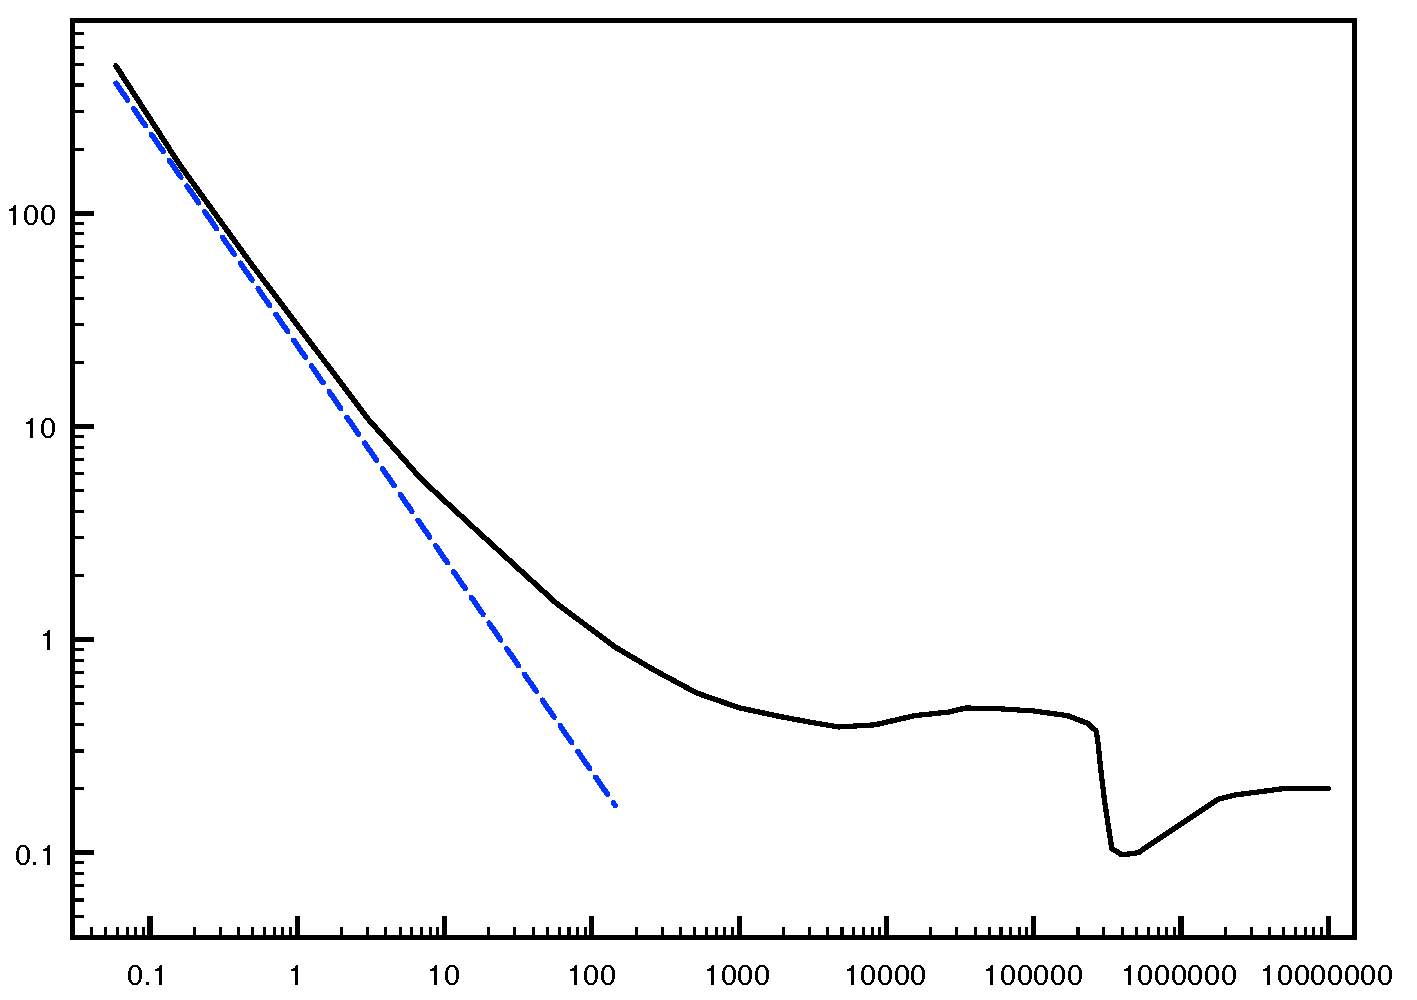
\includegraphics[width=70mm]{drag_coeff_sphere.pdf}}
		\put(0, 25){\begin{minipage}{20mm} \begin{center}
									Coefficient de traînée $$\color{rouge}
									C_d = \frac{F_x}{\frac{1}{2} \rho U^2 \, S}$$ \end{center}
								\end{minipage}}
		\put(35, -5){\begin{minipage}{50mm}
									Nombre de Reynolds \; $\color{bleu} Re = \frac{UD}{\nu}$
								\end{minipage}}
		\put(90, 15){\footnotesize $S = \pi R^2$ : surface projetée;}
		\put(90, 10){\footnotesize$U$ : vitesse incidente}
		\put(26, 10){\color{blue} \footnotesize  régime de Stokes $\dfrac{24}{Re}$}
		
		\put(88, 40){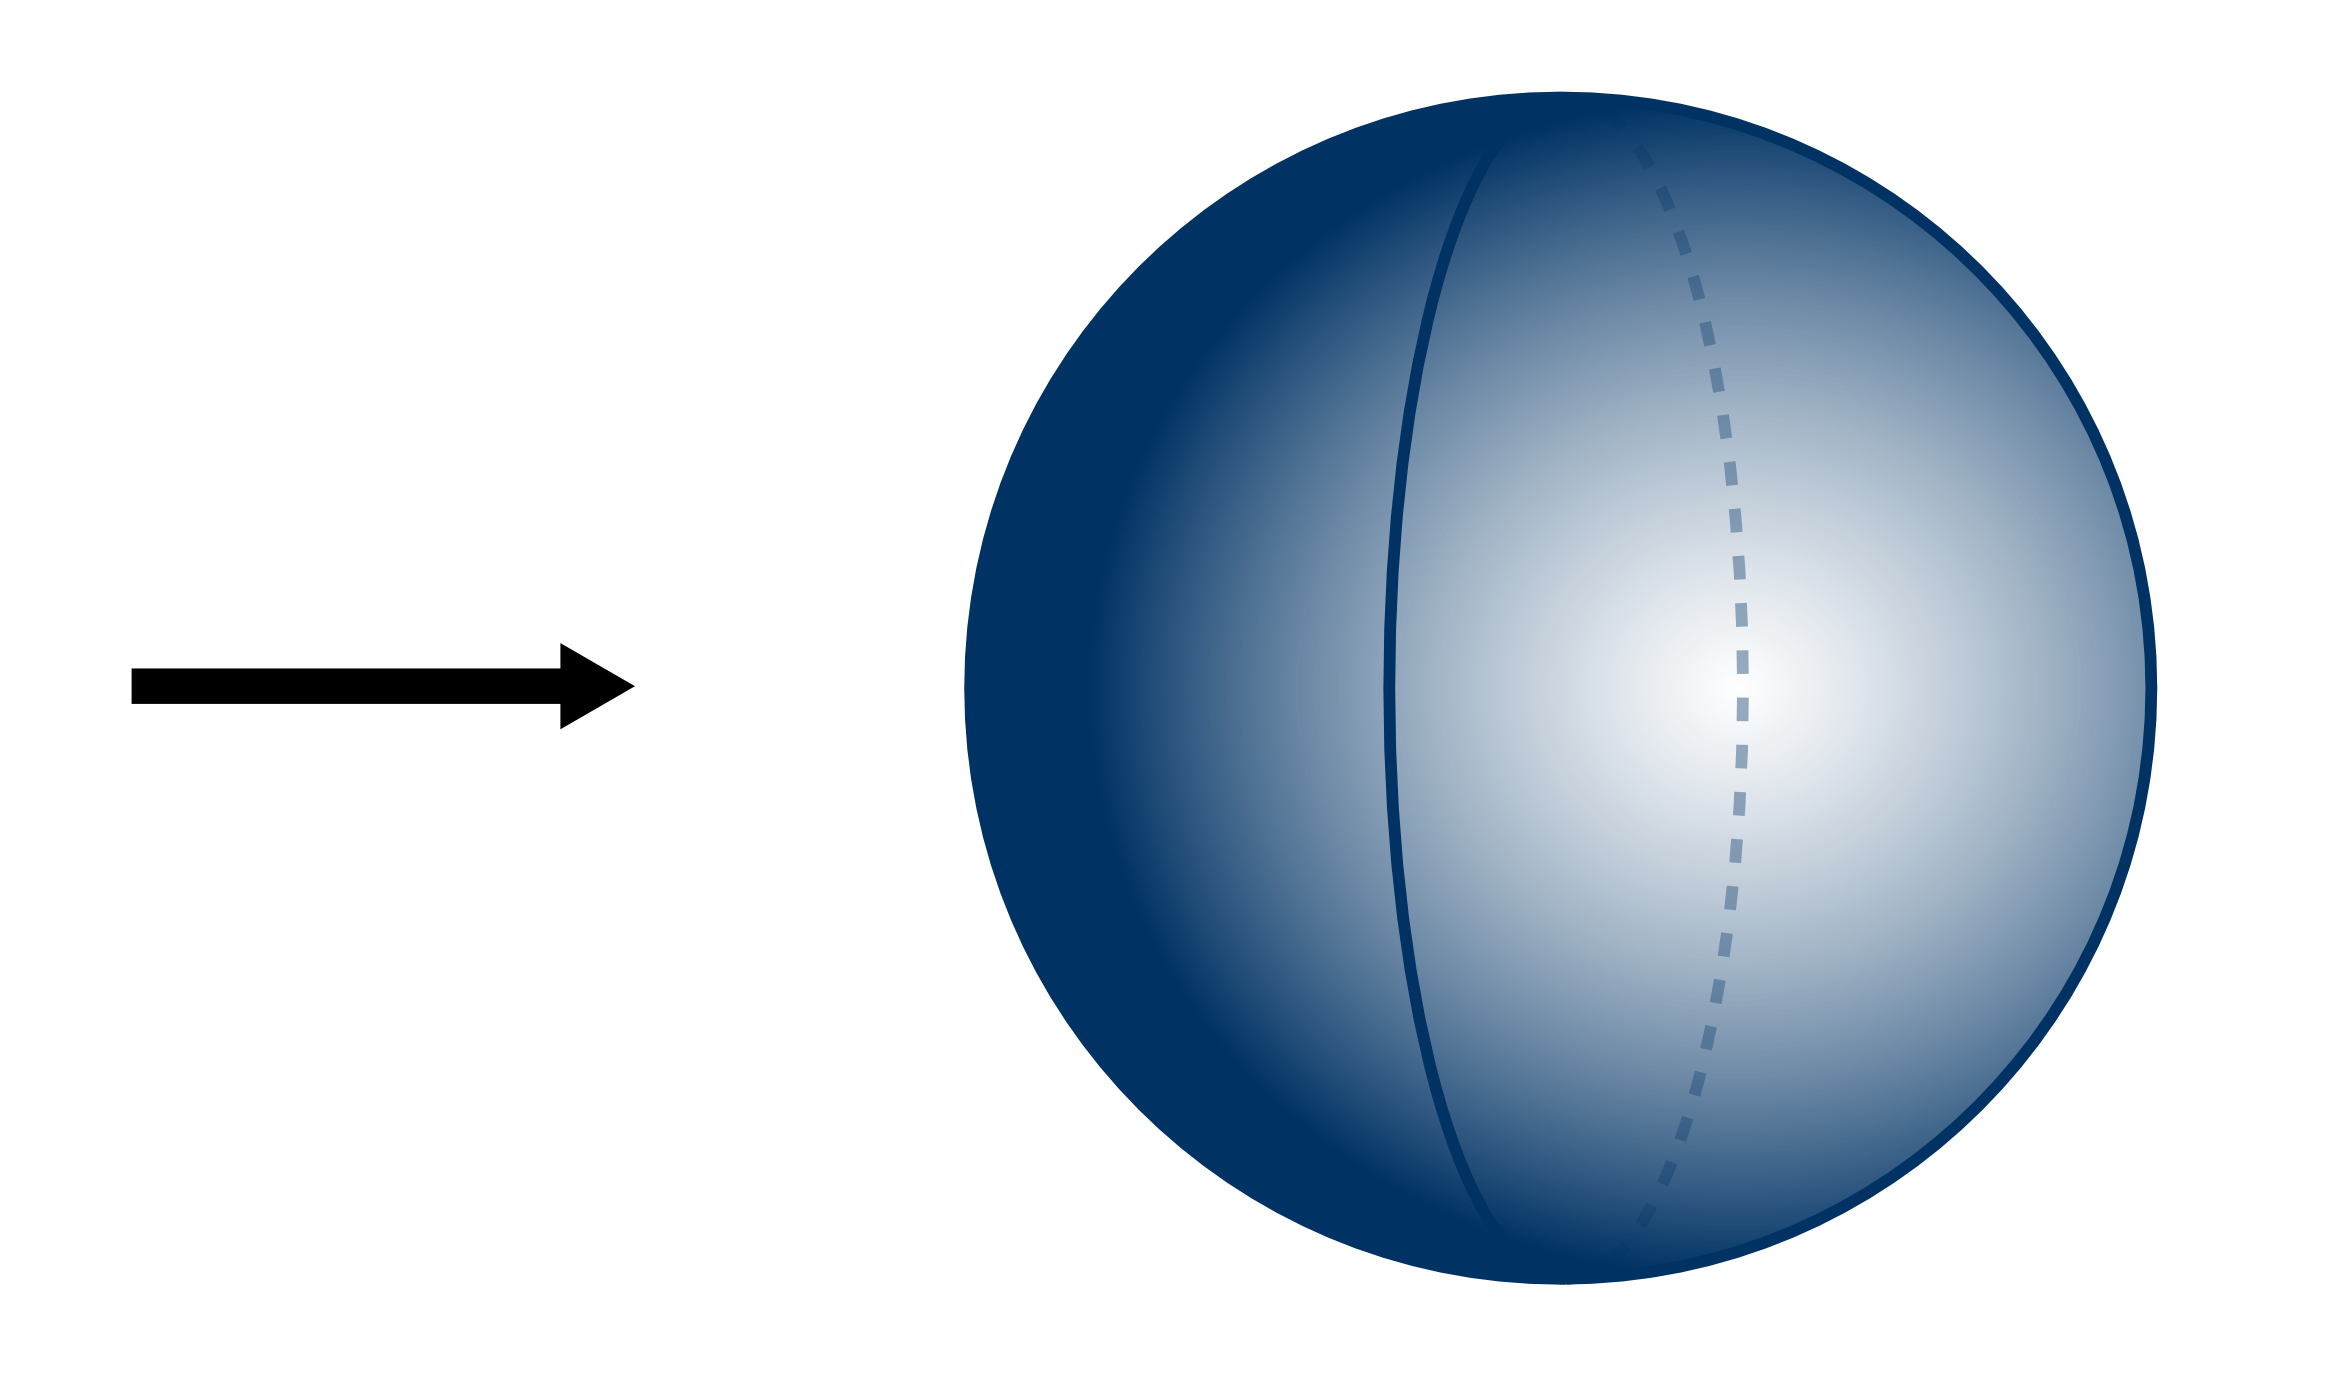
\includegraphics[width=25mm]{sphere.png}}
		\put(104.5, 47.5){\color{red} \vector(1, 0){10}}
		\put(112, 50){\color{red} $F_x$}

	\end{picture}
\end{center}


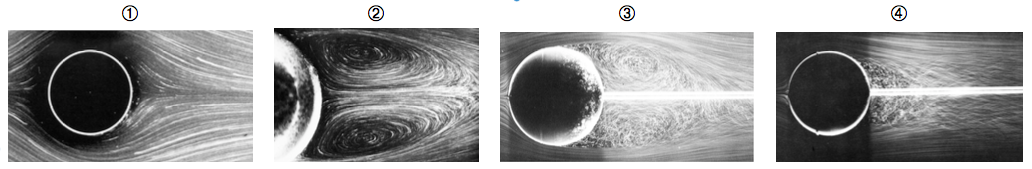
\includegraphics[width=100mm]{Sphere_Expe.png}



\vspace{0mm}

Illustrations : 
%\begin{verbatim} 
http://phylam.org/physique/resumes/resume-reynolds.pdf 
%\end{verbatim}

\end{frame}


%\begin{frame}{Structure de l'écoulement}
%\small

%\end{frame}

\begin{frame}{Ecoulement autour d'une sphère en mouvement oscillant}
\small

\textcolor{green}{Exercice (TD 9.1) : } 

Considérons une sphère de rayon $a$ oscillante à la pulsation $\omega$ :

$$\myvec{U} = U_0 \cos  (\omega t) \myvec{e}_x$$ 


On montre que sous les deux hypothèses :
\begin{itemize}
\item Oscillation de faible amplitude  ($U_0/\omega \ll a$),

\item Période d'oscillation rapide par rapport au temps de diffusion visqueuse  $(\omega^{-1} \ll \tau_v = a^2 / \nu )$,
\end{itemize}

Alors :

\begin{itemize}

\item 
Les effets visqueux restent confinés à une couche limite d'épaisseur $\delta = \sqrt{\nu/\omega}$.


\item 
A l'extérieur de la couche limite l'écoulement est potentiel et contribue à une force $\myvec{F}_p$ :
$$
\myvec{F}_p = - \rho V C \frac{d \myvec{U}}{d t} 
$$
où $V$ est le volume de la sphère et $C = 1/2$.

Interprétation : c'est la force a fournir pour accélérer une "masse ajoutée" à la sphère 
correspondant à un volume $V/2$ de fluide.

\item
Par analogie avec le second problème de Stokes (cf. TD 2) la force de frottement est 
$$
\myvec{F}_v  \approx - \frac{\mu a^2}{\delta} \myvec{U} 
$$

\end{itemize}

\end{frame}



\subsubsection{Exemple 3 : le profil d'aile}


%-----------------------------------------------------------------------------------------
\begin{frame}{Ecoulement autour d'un profil d'aile}
%-----------------------------------------------------------------------------------------

\small

%La \textcolor{rouge}{théorie de Prandtl (1905)}
%permet de décrire l'écoulement dans la couche limite en proche paroi.



	\begin{picture}(90, 0)(-9, 71)
		\put(0, 5){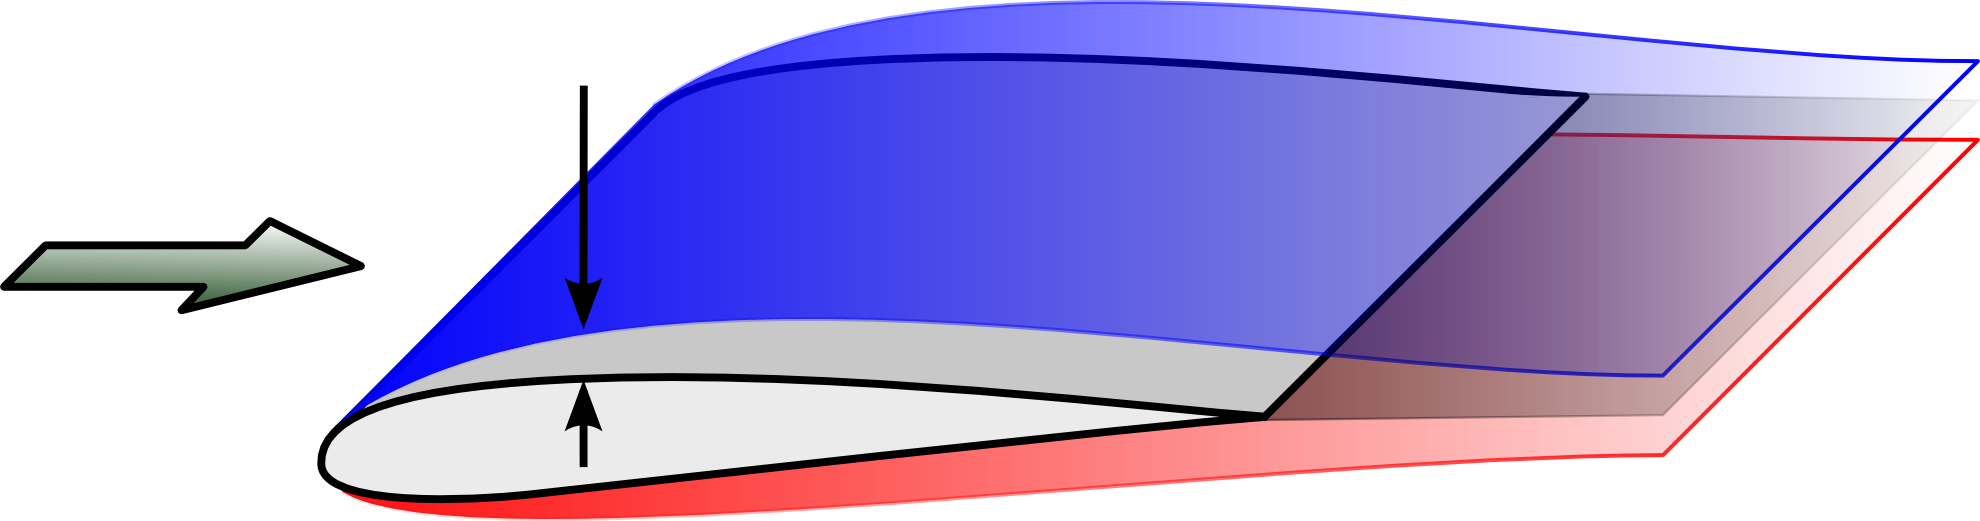
\includegraphics[width=60mm]{couche_limite_airfoil.png}}	
		\put(2, 23){couche limite}
		\put(2, 20){d'épaisseur $\delta \ll L$}
		\put(37, 30){\color{bleu} \vector(-1, -1){5}}
		\put(37,  4.5){\color{rouge} \vector(-1, 1){5}}
		\put(38, 3){\color{rouge} Solution intérieure : couche limite}
		\put(38, 29.5){\color{bleu} Solution extérieure : écoulement potentiel }
		\put(30, 9.3){\color{rouge} $\bullet$}
		\put(30, 24){\color{bleu} $\bullet$}
		\put(30, 1){\vector(-1, 0){20}}
		\put(30, 1){\vector(1, 0){10}}
		\put(23, 0){\colorbox{white}{$L$}}
	\end{picture}

\vspace{-1mm} \pause
On montre (cf. programme de master) que si l'angle d'incidence n'est pas trop élevé,
l'écoulement peut être décomposé en deux parties : \pause

\begin{itemize}
\item
Solution extérieure potentielle.

Peut être calculé à partir de la {\color{red} théorie des profils portants.}

\pause 
$\rightarrow$ permet de calculer la portance $F_y$. 


\item Solution intérieure visqueuse. 

Peut être calculée a partir de la {\color{red} théorie de la couche limite de Prandtl.}

\pause 
$\rightarrow$ permet de calculer la traînée $F_x$ 

\end{itemize}

\vspace{35mm}

\end{frame}

\begin{frame}{Notions sur la théorie des profils portants}

\small
Il existe des méthodes mathématiques puissantes pour calculer l'écoulement potentiel autour d'un objet 2D de forme quelconque (potentiel complexe, transformation conforme, ...) 

\smallskip
\pause
La solution n'est pas unique mais définie à une constante $\Gamma$ près (la circulation).
\smallskip
\pause
La "bonne" valeur de $\Gamma$ est celle qui conduit à un écoulement régulier au bord de fuite : condition de Kutta.

\pause
\begin{center}
\begin{tabular}{cc}
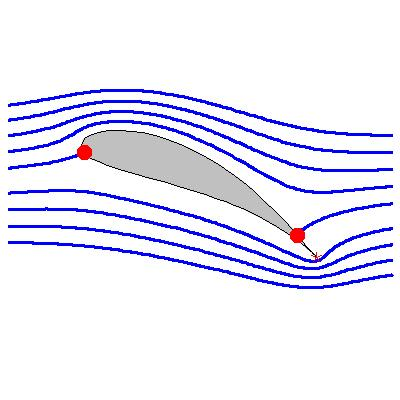
\includegraphics[width=30mm]{Figures/Joukowski.jpeg}
&
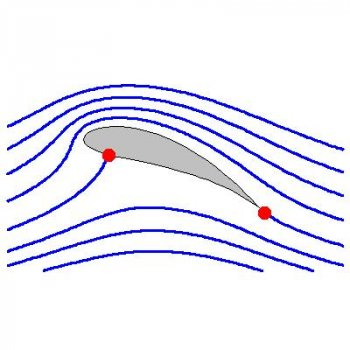
\includegraphics[width=30mm]{Figures/Joukowski_Kutta.jpeg}
\\
Solution avec $\Gamma = 0$ & Solution avec  $\Gamma \ne 0$ \\
Condition de Kutta non vérifiée & Condition de Kutta vérifiée
\end{tabular}
\end{center}

\pause
\smallskip
On montre que :
\begin{itemize}
\item Pour un profil symétrique $\Gamma = - \pi U L \alpha $ \quad $\rightarrow$ \quad 
$C_y = 2 \pi \alpha$
\item Pour un profil cambré $\Gamma = - \pi U L (\alpha-\alpha_0) $ \quad $\rightarrow$ \quad 
$C_y = 2 \pi (\alpha-\alpha_0)$

\end{itemize}
\end{frame}


%-----------------------------------------------------------------------------------------
\begin{frame}{Notions sur la théorie de Prandlt}
%-----------------------------------------------------------------------------------------
\small
La \textcolor{rouge}{théorie de Prandtl (1905)}
permet de décrire l'écoulement dans la couche limite en proche paroi.

%\vspace{-1mm} 

(cf. programme de master) : \pause

\small
	\begin{picture}(90, 0)(-9, 71)
		\put(0, 5){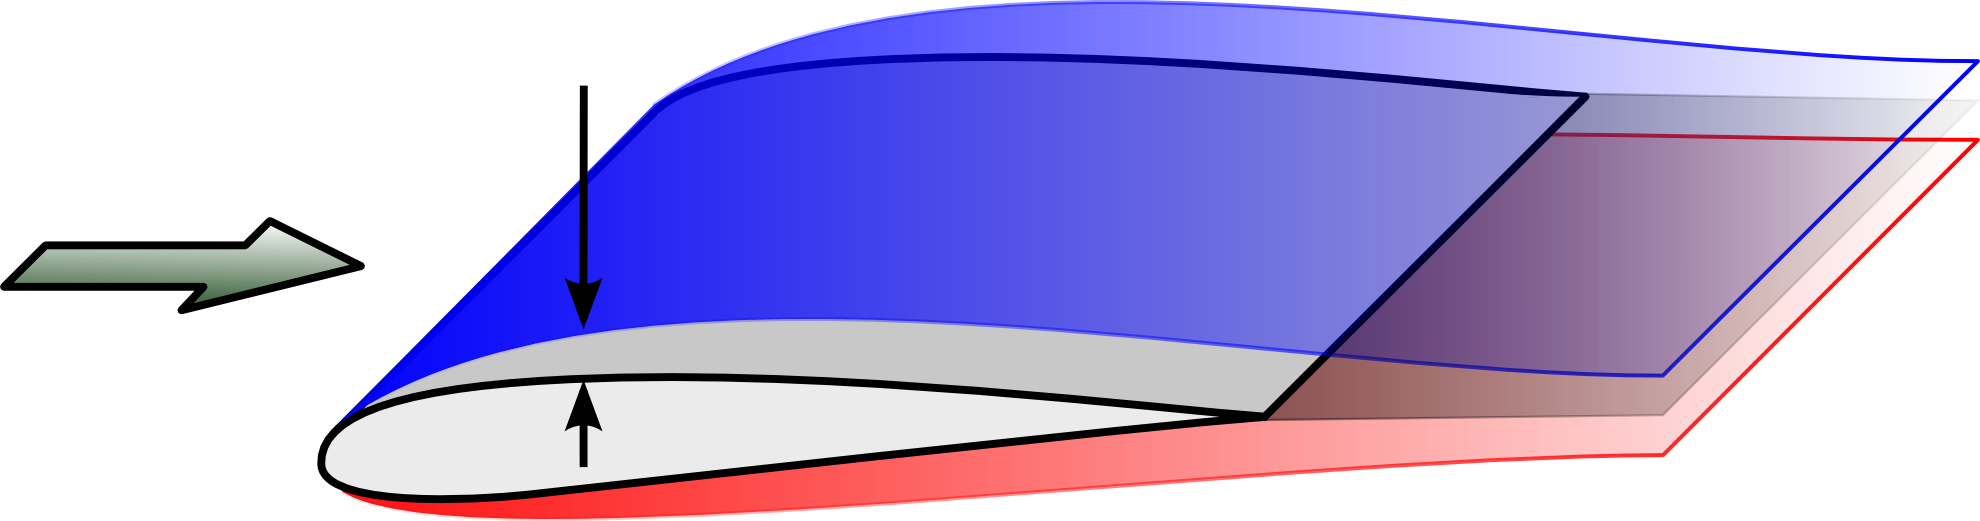
\includegraphics[width=60mm]{couche_limite_airfoil.png}}	
		%\put(2, 23){couche limite}
		%\put(2, 20){d'épaisseur $\delta \ll L$}
		%\put(37, 30){\color{bleu} \vector(-1, -1){5}}
		%\put(37,  4.5){\color{rouge} \vector(-1, 1){5}}
		%\put(38, 3){\color{rouge} Solution intérieure : couche limite}
		%\put(38, 29.5){\color{bleu} Solution extérieure : écoulement potentiel }
		%\put(30, 9.3){\color{rouge} $\bullet$}
		%\put(30, 24){\color{bleu} $\bullet$}
		%\put(30, 1){\vector(-1, 0){20}}
		%\put(30, 1){\vector(1, 0){10}}
		%\put(23, 0){\colorbox{white}{$L$}}
	\end{picture}

\vspace{-1mm} \pause

\begin{itemize}
\item
Si $Re < 10^5$  la couche limite est laminaire et est donnée par la solution de Blasius :

$$
\delta(x) \approx \sqrt{\nu x/U}
$$

\smallskip

Justification : analogie avec le problème de la couche limite temporelle sur une plaque infinie (premier problème de Stokes) pour lequel $\delta(t) = \sqrt{\nu t}$ (cf. chap. 2).
\smallskip

Dans ce cas la contrainte visqueuse est donnée par :
$
\tau_{xy}(x) = \mu \partial u / \partial y \approx \mu U / \delta(x)
$

\smallskip
et la force de frottement totale (linéique) vaut :
$
F_v = \int \tau_{xy}(x) dx  \approx \mu U \int_0^L (\nu x / U)^{-1/2} dx = \rho U^2 L Re^{-1/2}
$

\item Si $Re > 5 \cdot 10^5$ la couche limite est turbulente.

\smallskip
On utilise alors des lois empiriques pour estimer l'épaisseur des couches limites et la force de frottement. Par exemple : 

$$\delta(x) \approx 0.35 x \left( U x/\nu \right)^{-1/5}; 
\qquad 
F_v \approx \rho L U^2 \left( \log_{10}( Re )- 2 \right)^{-2}
$$

\end{itemize}

\vspace{35mm}

\end{frame}

%-----------------------------------------------------------------------------------------

%-----------------------------------------------------------------------------------------
\begin{frame}{Ecoulement autour d'un profil d'aile : cas des fortes incidences}
%-----------------------------------------------------------------------------------------

\small

\begin{center}
	\begin{picture}(90, 70)
		\put(0, 50){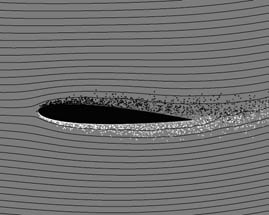
\includegraphics[width=25mm]{airfoil1.jpg}}
		\put(5, 48){\footnotesize incidence faible}
		\put(0, 25){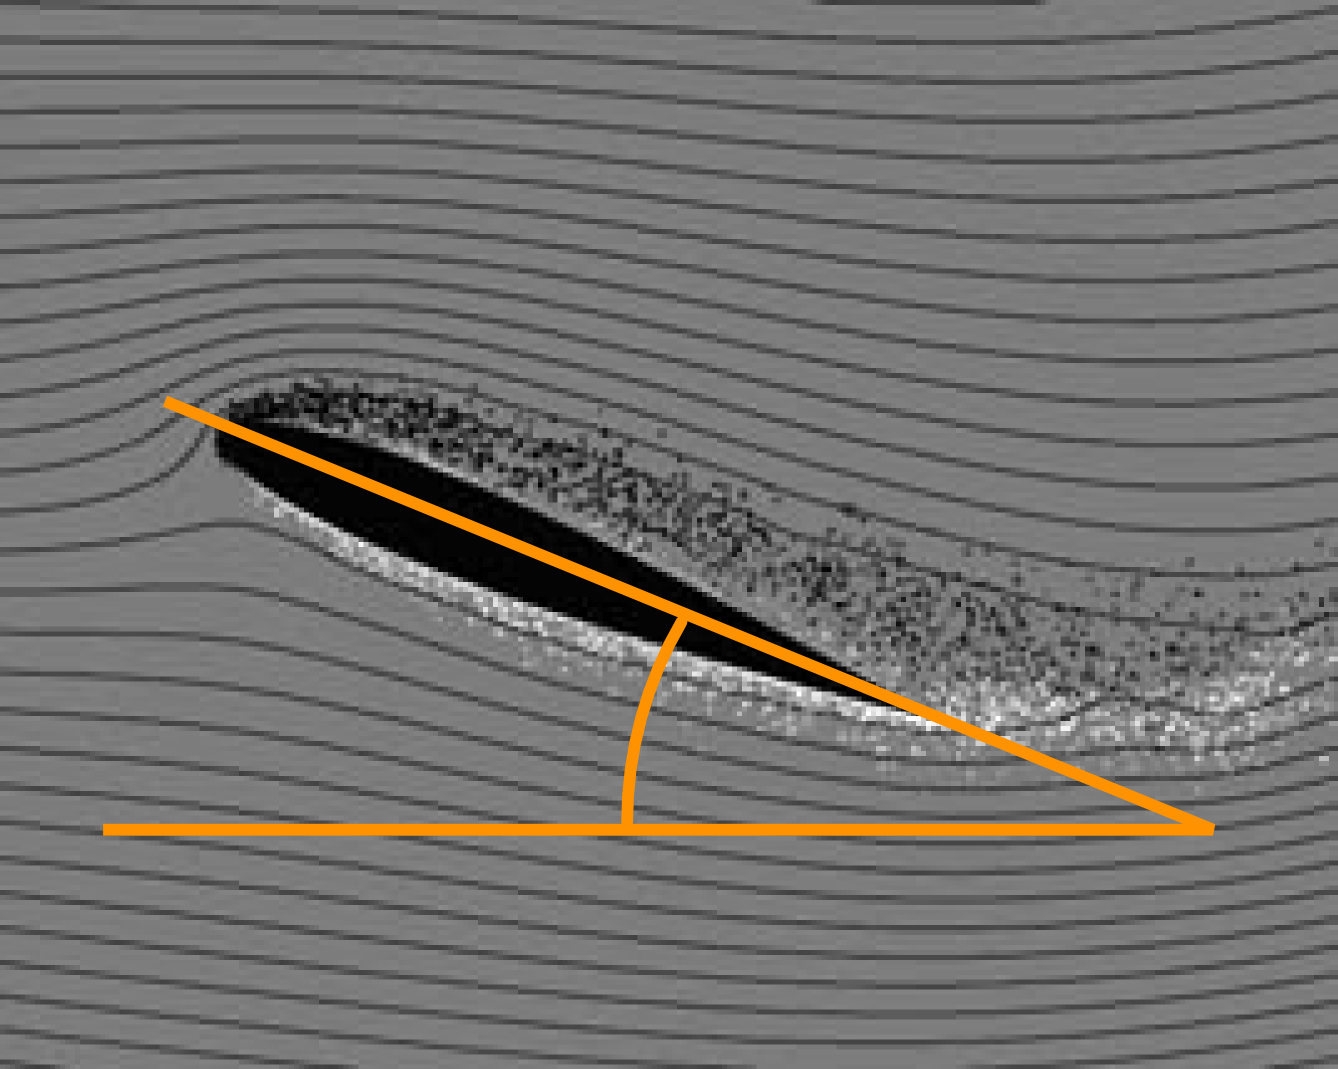
\includegraphics[width=25.1mm]{angle.png}}
		\put(5, 23){\footnotesize incidence modérée}
		\put(0, 0){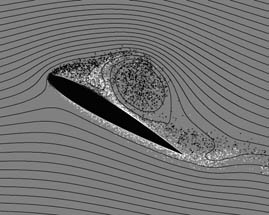
\includegraphics[width=25mm]{airfoil3.jpg}}
		\put(5, -2){\footnotesize incidence forte}
		\put(40, 5){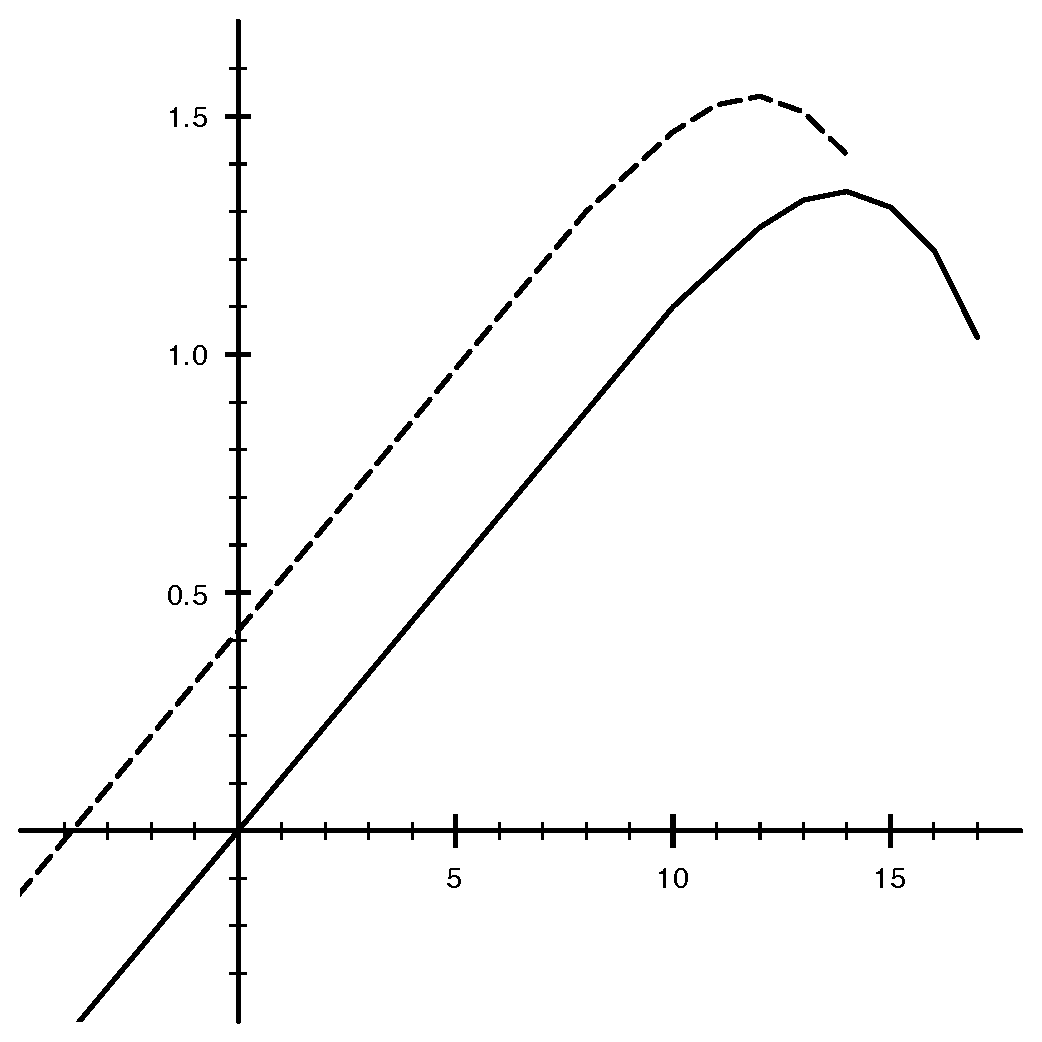
\includegraphics[width=50mm]{lift_coeff.pdf}}
		\put(75, 53){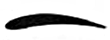
\includegraphics[width=10mm]{profil_cambre.png}}
		\put(85, 38){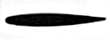
\includegraphics[width=10mm]{profil_non_cambre.png}}
		\put(8.5, 30.5){\setlength{\fboxsep}{0.3mm}\normalsize \colorbox{white}{\color{orange} $\alpha$}}
		\put(25, 60){\begin{minipage}{50mm} \begin{center}
									Coefficient de portance $$\color{rouge}
									C_L = \frac{F_z}{\frac{1}{2} \rho U^2 \, S}$$ \end{center}
								\end{minipage}}
		\put(60, 8){\begin{minipage}{50mm}
									Angle d'attaque \; $\color{bleu}\alpha$
								\end{minipage}}
		\put(82, 35){\footnotesize profil symétrique}
		\put(72, 58){\footnotesize profil cambré}
		\put(65, 32){\color{blue} \vector(0, 1){8}}
		\put(53, 48){\color{blue} \footnotesize  augmentation de}
		\put(53, 46){\color{blue} \footnotesize  la portance due}
		\put(53, 44){\color{blue} \footnotesize  à la cambrure}
		\put(80, 52){\color{red} \vector(0, -1){3}}
		\put(84.5, 49){\color{red} \vector(0, -1){5}}
		\put(81, 51.5){\color{red} \footnotesize décrochage dû au}
		\put(85.5, 49){\color{red} \footnotesize décollement}
		\put(55, 0){\footnotesize $S$ : surface de l'aile, $U$ : vitesse incidente}
		%\put(52.2, 12.5){\tiny 0}
		\put(80, 65){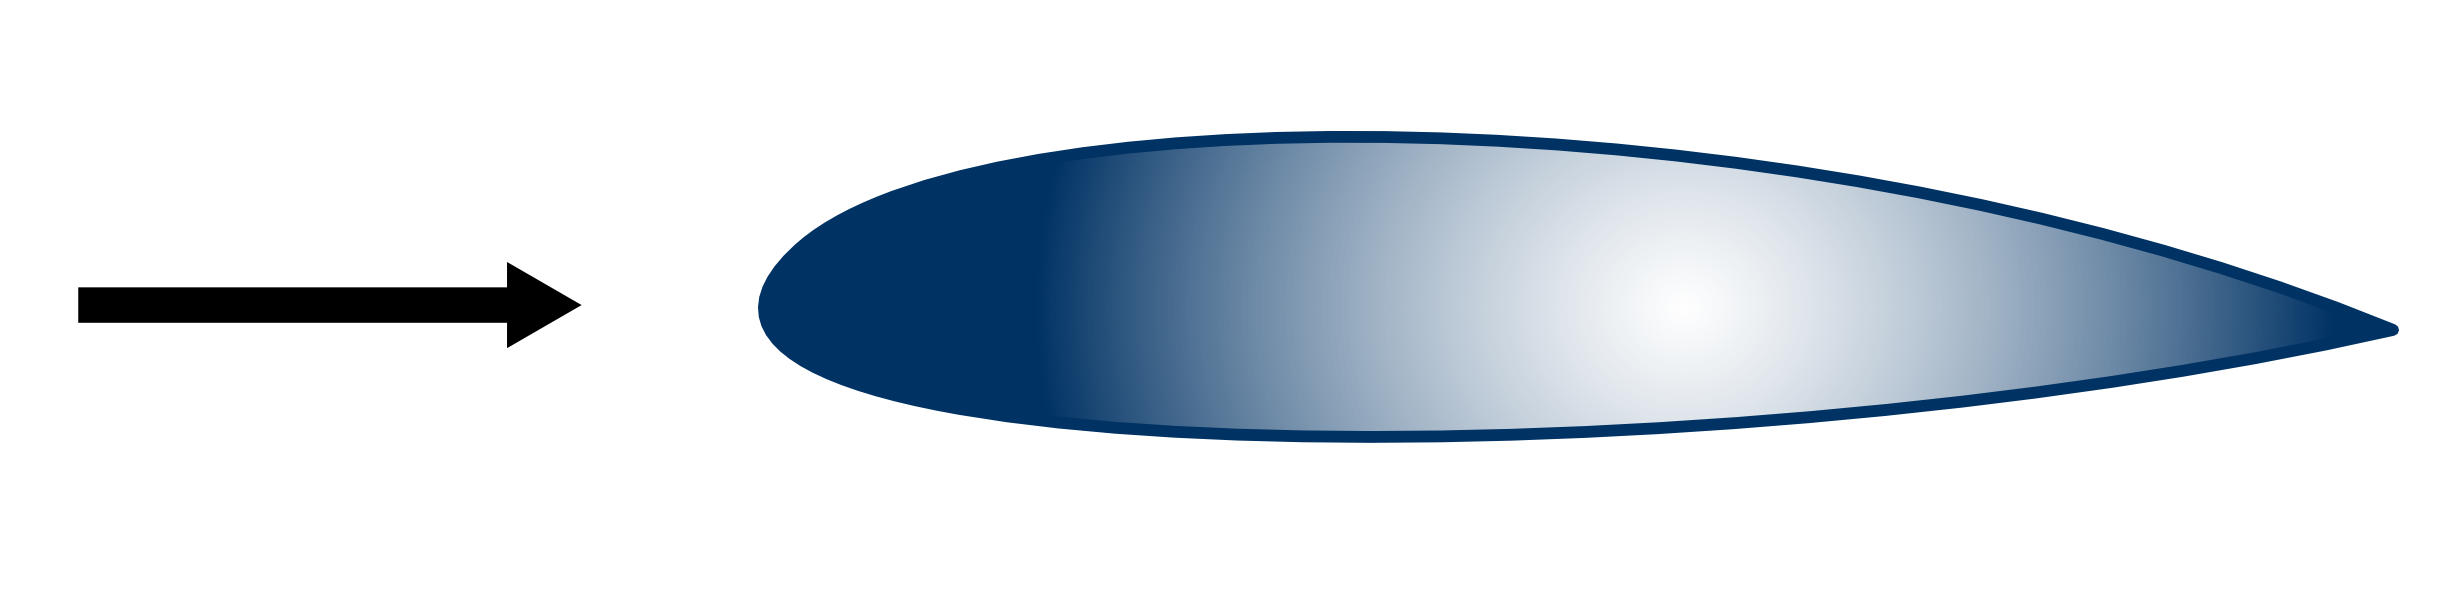
\includegraphics[width=25mm]{profil.png}}
		\put(95, 68){\color{blue} \vector(0, 1){7}}
		\put(90, 72){\color{blue} $F_z$}

	\end{picture}
\end{center}

\vspace{0mm}

\end{frame}

%\end{document}


\comment{
%-----------------------------------------------------------------------------------------
\begin{frame}{Notion de couche limite}
%-----------------------------------------------------------------------------------------

\small

La \textcolor{rouge}{théorie de Prandtl (1905)}
permet de décrire l'écoulement dans la couche limite en proche paroi.

	\begin{picture}(90, 0)(-9, 71)
		\put(0, 5){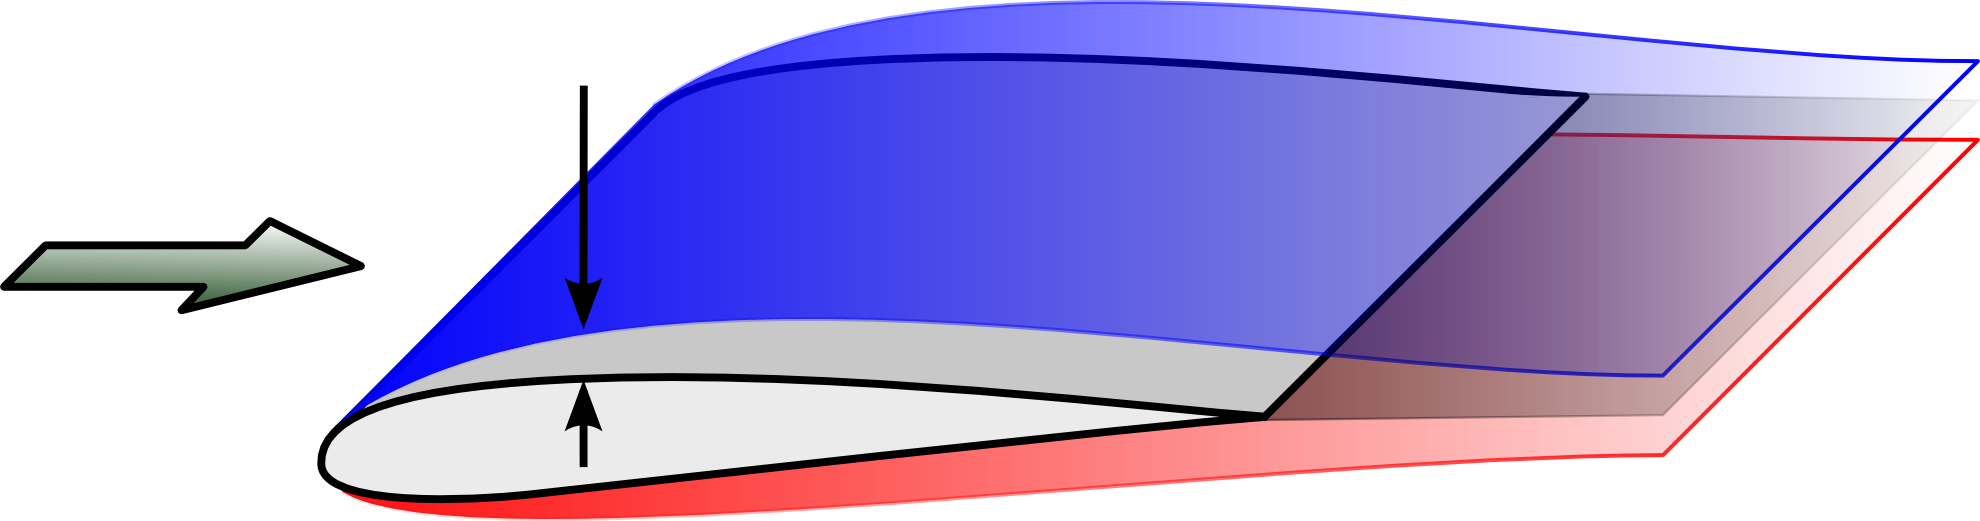
\includegraphics[width=60mm]{couche_limite_airfoil.png}}	
		\put(2, 23){couche limite}
		\put(2, 20){d'épaisseur $\delta \ll L$}
		\put(37, 30){\color{bleu} \vector(-1, -1){5}}
		\put(37,  4.5){\color{rouge} \vector(-1, 1){5}}
		\put(38, 3){\color{rouge} frottements visqueux non négligeables}
		\put(38, 29.5){\color{bleu} frottements visqueux négligeables : Euler OK}
		\put(30, 9.3){\color{rouge} $\bullet$}
		\put(30, 24){\color{bleu} $\bullet$}
		\put(30, 1){\vector(-1, 0){20}}
		\put(30, 1){\vector(1, 0){10}}
		\put(23, 0){\colorbox{white}{$L$}}
	\end{picture}

\vspace{-1mm} \pause
On montre (cf. programme de master) : \pause

\begin{itemize}
\item
	que la pression ne varie pas dans l'épaisseur de la couche limite :
	$
		\dfrac{\partial p}{\partial n} = 0
	$ \\ \vspace{-1mm}
	(où $n$ désigne la direction normale à la paroi)
	
	\pause 
	
	\vspace{-1mm}
\item
	que l'épaisseur de la couche limite à pour ordre de grandeur :
	$
		\delta = \dfrac{L}{\sqrt{Re}}, \quad\mbox{où $Re = UL/\nu$}
	$
\end{itemize}

\pause
On retrouve bien $\delta \ll L$ pour $Re\gg 1$ : l'approximation d'écoulement inertiel (ou de fluide parfait)
est donc valable sur un domaine qui coïncide quasiment avec l'intégralité du volume de fluide.

\medskip
\pause
Intérêt pratique en aérodynamique (par ex.) :
on calcule l'écoulement autour d'une géométrie d'aile
en fluide parfait et la pression calculée ainsi sur l'aile est correcte puisqu'elle ne varie pas à la traversée de la couche limite.

\vspace{35mm}

\end{frame}
}

